\documentclass[twoside]{projektInzynierskiMS1}
\usepackage{polski}
\usepackage[utf8]{inputenc}
\usepackage{amsmath}
\usepackage{graphicx}

\graphicspath{ {./images/} }
%\drukJednostronny

%% tytuł promotor iautor (\title to komenda standardowa)
\title{Automatyzacja procesów w przemyśle IT}
\promotor{dr inż. Zdzisław Sroczyński}


%% każdy autor musi mieć 3 argumenty: imię nazwisko, nr albumu, opis wkładu
\autor{Artur Kasperek}{1234}
\autor{Michał Płonka}{1234}
\autor{Patryk Musiol}{1234}

%% dedykacja mile widziana
% \dedykacja{To jest\\dedykacja}
%\NumeryNaPoczatku
%% numeracja wzorów tu włączona typu (1.2.3), ta druga to typu (1.2), domyślnie typu (1)
%\subsectionWzory
% \sectionWzory  

%\rozdzialy


%\literowaNumeracjaDodatkow %% włączy numerację dodatków literami
%\rzymskaNumeracjaDodatkow  %%włączy numerację dodatków liczbami rzymskimi

%% wyłączenie wyjaśnień:
\bezWyjasnien

%% standardowe komendy \newtheorem  działają jak woryginale
\newtheorem{tw}{Twierdzenie}%[subsection]
\newtheorem{twa}{Twierdzenie}%[section]
\newtheorem{dd}{Definicja}%[subsection]

\begin{document}
TODO dodać wstęp


\section{Automatyzacja a branża IT}
mógłbym tu opisać ogólnie całą branże IT oraz jak w przestrzeni lat ważny stał się CI/CD. Tutaj mógłbym umieścić trochę informacji o tym, że w projektach scrumowych szczególnie ważny jest CI/CD. Mógłbym opisać ogólnie, że dzisiaj dominują rozwiązania typu PaaS gdzie zespół nie musi już konfigurować od zera serwera CI/CD. Myślę że wstęp mógłby zawierać bardziej szczegółowe informacje o tym czym jest continues integration oraz czym jest continues delivery. Wydaje mi się, że nie ma sensu robić osobnego działu o tym czym te dwie rzeczy są, bo byłoby to lanie wody
\section{Wirtualizacja i orkiestracja}
myślę, że opisanie tego jak wirtualizacja pomaga w CI/CD zasługuje na swój rozdział. Szczególnie mógłbym ten rozdział poświęcić dockerowi z faktu, że zdominował rynek. Warto tutaj byłoby napisać też o rozwiązaniach które były używane w przeszłości a zostały wyparte jak vagrant. Dodatkowo w rozdziale mozemy opisać na czym polega orkiestracja - Kubernates, docker swarm
\section{Hudson oraz Jenkins - klasyczne narzędzia do CI/CD}
tutaj mógłbym zamieścić trochę informacji historycznych jak język java zrewolucjonował inżynierię oprogramowania i dalej rozwinąć, że pokłosiem tego było powstanie Jenkinsa. Myślę, że mógłbym tutaj opisać najbardziej uniwersalne rzeczy które są w nim używane. Wydaje mi się że mógłbym poszukać alternatyw do Jenkinsa by rozszerzyć ten dział.
Jako część tego rozdziału mógłbym zawrzeć problem gdzie konieczne jest użycie Jenkinsa i to byłoby zrobione jako część praktyczna. Wbrew pozorom do niektórych zastosować Jenkins nadal jest używany, np do środowisk gdzie QA musi odpalać środowisko z różnymi parametrami
\section{Platformy SaaS z wbudowanym CI/CD}
\subsection{Z czego wynika popularność platform SaaS?}
Platformy takie jak GitHub, CircleCI czy też BitBucket zasłynęły z tego, że oferowały możliwość hostowania naszego repozytorium Git'owego w chmurze. Z biegiem czasu zaczęły one oferować dodatkowe usługi. Serwisy te to już nie tylko miejsce, które umożliwia hostowanie naszego repozytorium kodu - pozwalają one na takie rzeczy jak:
\begin{itemize}
    \item Uruchamianie procesów automatyzujących (GitHub, GitLab, BitBucket) - dzięki możliwości tworzenia własnych procesów automatyzujących mamy możliwość zaimplementować własny proces ciągłej integracji, ciągłego dowożenia czy też ciągłego dostarczania,
    \item Uruchamianie manualne predefiniowanych procesów (GitLab) - jest to dość prosta funkcjonalność, która daje sporo możliwości. GitLab dostarcza interfejs, w którym możemy uruchomić dowolny pipeline (z ang. \textit{potok}) manualnie - dodatkowo możemy podać argumenty w postaci pól tekstowych. Przykładem, gdzie ta funkcja GitLab'a byłaby użyteczna, jest aplikacja webowa, która zabiera dużo zasobów. Użycie procesu ciągłego dostarczania, by uruchamiać wersję staging'ową oznaczałoby, że aplikacja ta zbędnie używałaby zasoby na serwerze. Dzięki funkcji uruchamiania manualnego pipeline'ów moglibyśmy uruchamiać aplikację tylko wtedy, kiedy chcielibyśmy przetestować jak działa,
    \item Integracja z Kubernetes'em (GitLab) - GitLab upraszcza proces release'u naszego oprogramowania dzięki integracji z Kubernetes'em. Możemy podpiąć istniejący już klaster albo stworzyć nowy. GitLab może stworzyć taki klaster za nas pod warunkiem, że będzie on działał na chmurze AWS albo Google Cloud,
    \item Publikacje strony statycznej (GitHub) - GitHub umożliwia publikacje danego folderu z plikami statycznymi strony internetowej, który jest częścią repozytorium. Dzięki temu możemy uprościć proces publikacji naszej strony internetowej,
    \item Hosting obrazów Docker'owych oraz paczek / bibliotek (GitHub, GitLab, BitBucket) - dzięki hostingowi obrazów Docker'owych możemy uprościć proces późniejszego uruchomienia naszego kodu na serwerze. Dodatkowo możemy hostować na tych platformach paczki popularnych języków. Wspierane są między innymi: NPM (nodeJS), Maven (Java), NuGet (.NET), RubyGems (Ruby),
    \item Śledzenia zadań (GitHub, GitLab, BitBucket) - każda ze znaczących platform ma wbudowane w sobie oprogramowanie do śledzenia zadań. Dzięki temu możemy stworzyć prostą metodykę Agile'ową używając tego, co zapewnia nam dana platforma. Z reguły oprogramowanie to jest mocno ograniczone i nadaje się do prostszych projektów. Zespoły, które mają większe wymagania, muszą szukać oddzielnego oprogramowania,
    \item Audyt bezpieczeństwa bibliotek (GitHub, GitLab) - dzięki tej funkcjonalności możemy się dowiedzieć, czy nasze zależności trzecie nie posiadają luk bezpieczeństwa. GitHub lub GitLab w przypadku wykrycia takiego problemu wysyła maila z powiadomieniem oraz tworzy automatyczną poprawkę,
    \item Sponsoring (GitHub) - GitHub posiada wbudowaną opcję która włącza sponsoring naszego projektu. Dzięki temu na stronie głównej repozytorium pojawia się ikonka serca, która pozwala wesprzeć dany projekt pieniężnie. Jest to ciekawa opcja dla projektów open source.
\end{itemize}
Powyższe funkcjonalności czynią te platformy narzędziami all-in-one (z ang. wszystko w jednym). Dzięki temu, że są one oferowane jako serwisy SaaS, czas który musimy poświęcić na utrzymanie i instalację ogranicza się do zera.
\par
Należy pamiętać, że użycie platform SaaS ma dwie strony medalu. Jeżeli nasz projekt jest publiczny, większość z powyższych usług jest oferowana za darmo. Natomiast jeżeli nasz projekt posiada kod, który jest prywatny, będziemy musieli uiścić odpowiednią opłatę. Zazwyczaj opłata ta jest uzależniona od liczby usług, z których będziemy korzystać oraz od minut automatycznych procesów, które zużyjemy. Platformę na której będziemy działać należy dobrać do indywidualnych potrzeb danego projektu - każda z nich oferuje swoiste ekskluzywne funkcjonalności. Jeżeli naszym celem jest stworzenie statycznej strony, najlepszym wyborem wydaje się GitHub, który oferuje darmowy hosting. Z drugiej strony jeśli zależy nam na uruchamianiu procesów automatyzujących manualnie to powinniśmy spojrzeć w stronę GitLab'a. GitHub jest świetnym rozwiązaniem dla projektów open source, ponieważ większość dodatkowych usług dla takich projektów jest oferowana za darmo. Wynika to z polityki, która została obrana przez właściciela - Microsoft.
\subsection{Strona statyczna - przykład użycia GitHub Actions i GitHub Pages}
Załóżmy, że chcielibyśmy stworzyć stronę internetową, która pozwoliłaby nam przedstawić kim jesteśmy. Mamy następujące wymagania:
\begin{itemize}
    \item Strona ma być statyczna. Dzięki temu będziemy mogli wykorzystać hosting plików, który często jest oferowany jako darmowa opcja,
    \item Strona powinna mieć co najmniej dwie podstrony, które zawierają wspólne sekcje: nagłówek oraz stopkę,
    \item Strona ma być dostępna w sieci za pomocą promowanego przez przeglądarki protokołu HTTPS.
\end{itemize}
By ułatwić sobie powyższe zadanie, użyjemy framework'a Gatsby.js. Jest to generator stron statycznych, który upraszcza tworzenie takowych stron. Framework używa popularną bibliotekę React, która pozwala korzystać z składni JSX (składnia mocno przypomina format HTML). Główną cechą Gatsby'iego jest to, że zapewnia integracje z popularnymi systemami takimi jak Wordpress \cite{GatsbyJSWordpress}. Dzięki temu nie jesteśmy zmuszeni utrzymywać dedykowanego serwera PHP - Gatsby wygeneruje wszystkie możliwe podstrony podczas procesu budowania strony. Jest to szczególnie ciekawe rozwiązanie dla serwisów, które generują duży ruch. Znacznie łatwiej serwować pliki statyczne niż za każdym razem budować stronę, obciążając dodatkowo bazę danych.
\par
Gatsby.js w postaci programu działającego w wierszu poleceń pozwala w prosty sposób pobrać startowy szablon z minimalnym zbiorem potrzebnych rzeczy. Użyjmy tego szablonu jako punktu wejściowego:
\begin{lstlisting}[caption={Pobierania szablonu startowego}]
    gatsby new static-website-with-ci-cd https://github.com/gatsbyjs/gatsby-starter-default
\end{lstlisting}
Domyślny szablon posiada w dużej mierze gotowy layout z nagłówkiem oraz stopką. Jest on zdefiniowany w pliku 'src/components/layout.js'. Po małej przeróbce wygląda on następująco:
\begin{lstlisting}[caption={Layout - komponent zawierający logikę związaną z layoutem strony}]
    const Layout = ({ children }) => {
        const data = useStaticQuery(graphql`
          query SiteTitleQuery {
            site {
              siteMetadata {
                title
              }
            }
          }
        `)
      
        return (
          <>
            <Header siteTitle={data.site.siteMetadata?.title || `Title`} />
            <div
              style={{
                margin: `0 auto`,
                maxWidth: 960,
                padding: `0 1.0875rem 1.45rem`,
              }}
            >
              <main>{children}</main>
              <footer style={{
                marginTop: `2rem`
              }}>
                Stopka
              </footer>
            </div>
          </>
        )
    }
\end{lstlisting}
Dzięki temu, że zawartość sekcji \textit{$<$main$>$} jest konfigurowalna za pomocą argumentu \textit{children}, możemy współdzielić layout między różnymi podstronami.
\par
Pierwszą stroną, którą chcielibyśmy stworzyć, jest strona domowa. Na niej wyświetlimy podstawowe informacje o nas oraz umieścimy link do strony, na której przedstawimy więcej danych o sobie. Kod tej strony jest stosunkowo prosty:
\begin{lstlisting}[caption={index.js - plik zawiera treść strony domowej}]
  import React from "react"
  import { Link } from "gatsby"
  import Layout from "../components/layout"
  import SEO from "../components/seo"
  import MeImgSrc from "../images/ja.jpg"

  const IndexPage = () => (
    <Layout>
      <SEO title="Home" />
      <div>
        <h2>Artur Kasperek - Programista oraz Student Politechniki Slaskiej</h2>
        <img src={MeImgSrc}/>
      </div>
      <div>
        <Link to="/detale">Wiecej o mnie</Link> <br />
      </div>
    </Layout>
  )

  export default IndexPage
\end{lstlisting}
Drugą stroną jest podstrona, która wyświetla więcej szczegółów. Podobnie jak na stronie domowej zawiera link do głównej strony. Zawartość wygląda następująco:
\begin{lstlisting}[caption={detale.js - plik zawiera treść strony z szczegółami}]
  import React from "react"
  import { Link } from "gatsby"

  import Layout from "../components/layout"
  import SEO from "../components/seo"

  const SecondPage = () => (
    <Layout>
      <SEO title="Detale" />
      <h2>Doswiadczenie</h2>
      <ul>
        <li>JavaScript</li>
        <li>HTML</li>
        <li>CSS</li>
        <li>C++</li>
        <li>NodeJS</li>
      </ul>
      <h2>Szkoly</h2>
      <ul>
        <li>Politechnika Slaska</li>
        <li>I Liceum Ogolnoksztalcacego im. Stefana Zeromskiego w Zawierciu</li>
        <li>Gimnazjum nr 1 Zawierciu</li>
      </ul>
      <Link to="/">Powrot do strony domowej</Link>
    </Layout>
  )

  export default SecondPage

\end{lstlisting}
\par
Strona może być teraz opublikowana. Do tego celu służy komenda \textit{gatsby build}. Komenda ta buduje stronę i umieszcza ją w folderze \textit{public}. Chcielibyśmy teraz w jakiś sposób opublikować stronę w sieci. W tym celu możemy skorzystać z usługi GitHub Pages. Wymogiem jest tutaj to, by nasz kod strony internetowej był repozytorium Git'owym trzymanym na GitHub'ie. Po tym, gdy nasz projekt jest już repozytorium Git'owym na GitHub'ie, możemy stworzyć definicję potoku ciągłego dowożenia. Chcielibyśmy, by za każdym razem, gdy nowy kod zostaje wysłany na gałąź \textit{master}, strona się budowała i była publikowana w sieci.
\par
GitHub Actions posiada własną składnię do definicji potoków automatyzujących. Najmniejszą jednostką, którą możemy zdefiniować jest \textit{workflow} (z ang. \textit{przepływ}). W dokumentacji \cite{GithubActionsDoc} możemy dowiedzieć się, że \textit{workflow} to konfigurowalny zautomatyzowany proces składający się z co najmniej jednego zadania oraz pliku YAML, który zawiera jego definicję. Warto podkreślić, że plik ten jest częścią naszego projektu - wynika z tego, że jest on wersjonowany wraz z kodem źródłowym i innymi plikami.
\par
Plik YAML danego \textit{workflow} zawiera informację o swojej nazwie, to kiedy ma się uruchomić oraz definicję tego co ma wykonać. W naszym przypadku chcemy, by nasz \textit{workflow} wykonywał się za każdym razem, gdy wrzucamy jakieś zmiany na master'a. Możemy to osiągnąć za pomocą poniższego fragmentu kodu:
\begin{lstlisting}[caption={Nazwa oraz definicja wyzwalacza \textit{workflow} budującęgo stronę}]
  name: Build and Deploy

  on:
    push:
      branches: [ master ]
\end{lstlisting}
\par
Kolejnym krokiem jest zdefiniowanie to, co nasz \textit{workflow} ma robić. W naszym przypadku chcielibyśmy zbudować stronę oraz opublikować ją za pomocą GitHub Pages. W tym celu w ustawieniach projektu włączamy GitHub Pages oraz definiujemy, w jakim folderze oraz na jakiej gałęzi będą dostępne pliki statyczne strony. W naszym przypadku wybieramy gałąź \textit{gh-pages} oraz główny folder.
\begin{figure}[htbp]
  \centering
  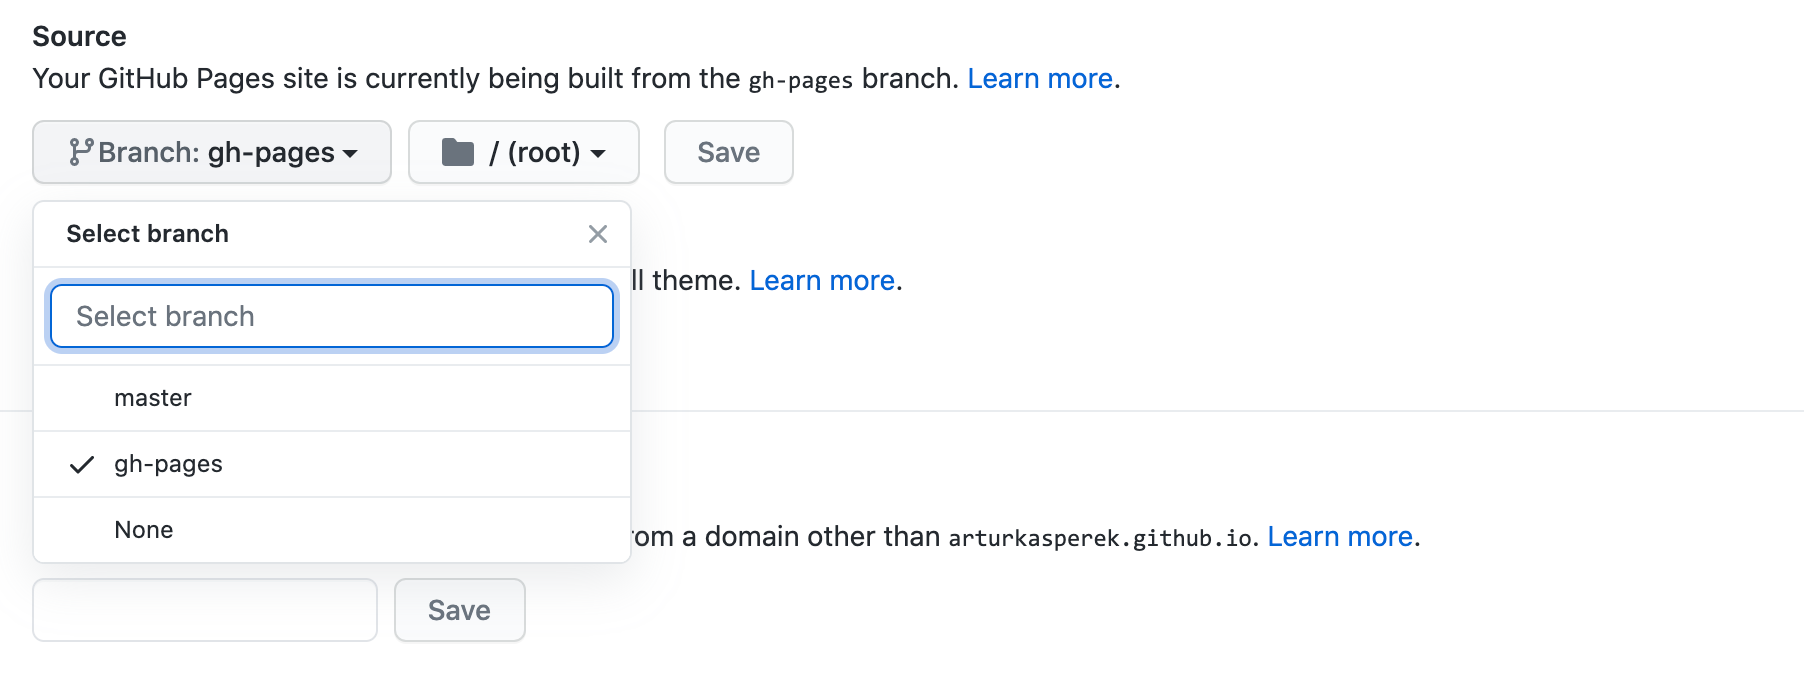
\includegraphics[width=12cm]{gh_pages.png}
  \caption{Ustawienia GitHub Pages}
  \label{fig:gh_pages}
\end{figure}
Dzięki temu będziemy w stanie odseparować gałąź, gdzie trzymamy kod źródłowy strony, od zbudowanej statycznej strony. Jest to także ułatwienie dla potoku automatyzującego. Jeżeli chcielibyśmy zapisywać zbudowaną stronę na gałęzi \textit{master}, oznaczałoby to, że nasz \textit{workflow} wyzwalałby się w nieskończoność przez fakt, iż jest on uzależniony od tego, czy jakieś nowe zmiany zostały wysłane na gałąź \textit{master}.
\par
Definicja tego, co nasz proces ciągłego dowożenia ma robić, wygląda następująco:
\begin{lstlisting}[caption={Definicja zadań \textit{workflow}'a budującego stronę}]
  jobs:
    build-and-deploy:
      runs-on: ubuntu-latest
      steps:
      - uses: actions/checkout@v2
      - name: Use Node.js 14.x
        uses: actions/setup-node@v1
        with:
          node-version: 14.x
      - name: Install Dependencies
        run: |
          yarn install
      - name: Build website
        run: |
          yarn build
      - name: Deploy
        uses: JamesIves/github-pages-deploy-action@3.6.2
        with:
          GITHUB_TOKEN: ${{ secrets.GITHUB_TOKEN }}
          BRANCH: gh-pages
          FOLDER: public
          CLEAN: true
\end{lstlisting}
\par
Jedną z rzeczy, które wyróżniają GitHub Actions nad innymi systemami ciągłej integracji/ciągłego dowożenia, jest możliwość definiowania tytułowych akcji. Akcje to nic innego jak sprytnie zapakowane programy lub też skrypty bash'owe, które pod spodem wykonują jakąś skomplikowaną rzecz. W zależności od argumentów środowiskowych możemy daną akcję dostosować do naszych potrzeb. Z faktu, że każdy może publikować własne akcje, nie jesteśmy ograniczeni do korzystania tylko z akcji dostarczonych przez twórców GitHub Actions. Dzięki takiemu podejściu mamy dostęp do bogatej bazy gotowych modułów.
\par
Wyjaśnijmy teraz, co dane linijki robią. W linii 3 definiujemy to, jaki system chcemy użyć jako bazowy. W naszym przypadku używamy Ubuntu, ponieważ jest najbardziej „lekkim” z wszystkich możliwych systemów. Od linijki 4 do końca mamy definicję kroków, co dany \textit{job} (z ang. \textit{zadanie}) ma wykonać. Pierwszymi krokami jest przełączenie się do danego branch'a oraz użycie akcji, która zainstaluje nam środowisko nodeJS w wersji 14. Od linii 10 do 15 zdefiniowane są dwa kroki, których celem jest zainstalowanie zależności naszego projektu oraz jego zbudowanie. W tym celu używamy menadżera paczek \textit{yarn}, który został zainstalowany dodatkowo podczas instalacji nodeJS. Kroki te pokazują, że nie jesteśmy uzależnieni tylko od użycia gotowych akcji. Za pomocą słowa kluczowego \textit{run} możemy zdefiniować dowolną komendę bash'ową, która ma być wykonana w danym momencie. Warto podkreślić fakt, że zmienne środowiskowe, które były zdefiniowane w danym kroku, nie są dostępne dla kolejnych kroków. GitHub Actions uruchamia każdy krok w osobnej sesji bash'owej. Na ten moment nasza strona powinna być wybudowana i zapisana w folderze \textit{public}.
\par
Ostanim krokiem jest publikacja strony na gałęzi \textit{gh-pages}. W tym celu używamy gotowej akcji o nazwie \textit{JamesIves/github-pages-deploy-action} w wersji 3.6.2. Jest to przykład akcji, która została dostarczona przez trzeciego autora i jest udostępniona szerokiej publiczności. Akcja ta „pod spodem” za pomocą git'a wysyła dany folder na wyspecjalizowaną za pomocą parametru \textit{BRANCH} gałąź. Dodatkowo musimy podać w parametrach akcji token dostępu do GitHuba. Robimy to za pomocą parametru \textit{GITHUB\_TOKEN}. Token ten jest automatycznie generowany przez GitHub'a podczas uruchamiania danego \textit{workflow}'a i daje możliwość zapisywania zmian do repozytorium, gdzie \textit{workflow} jest uruchamiany. Tym sposobem akcja dostaje niezbędne prawa do wysłania folderu z wybudowaną stroną na gałąź \textit{gh-pages}, która jest częścią tego samego repozytorium. Dzięki temu, że wykorzystaliśmy gotową akcję do publikacji naszej strony, ograniczyliśmy długość kodu oraz zredukowaliśmy czas, który musielibyśmy poświęcić na stworzenie skryptu, który wysyła folder \textit{public} na odpowiednią gałąź.
\par
Teraz, gdy nasze repozytorium posiada plik konfiguracyjny GitHub Actions, w zakładce \textit{Action} na GitHub'ie powinniśmy zauważyć zakolejkowane zadanie budowania strony.
\begin{figure}[htbp]
  \centering
  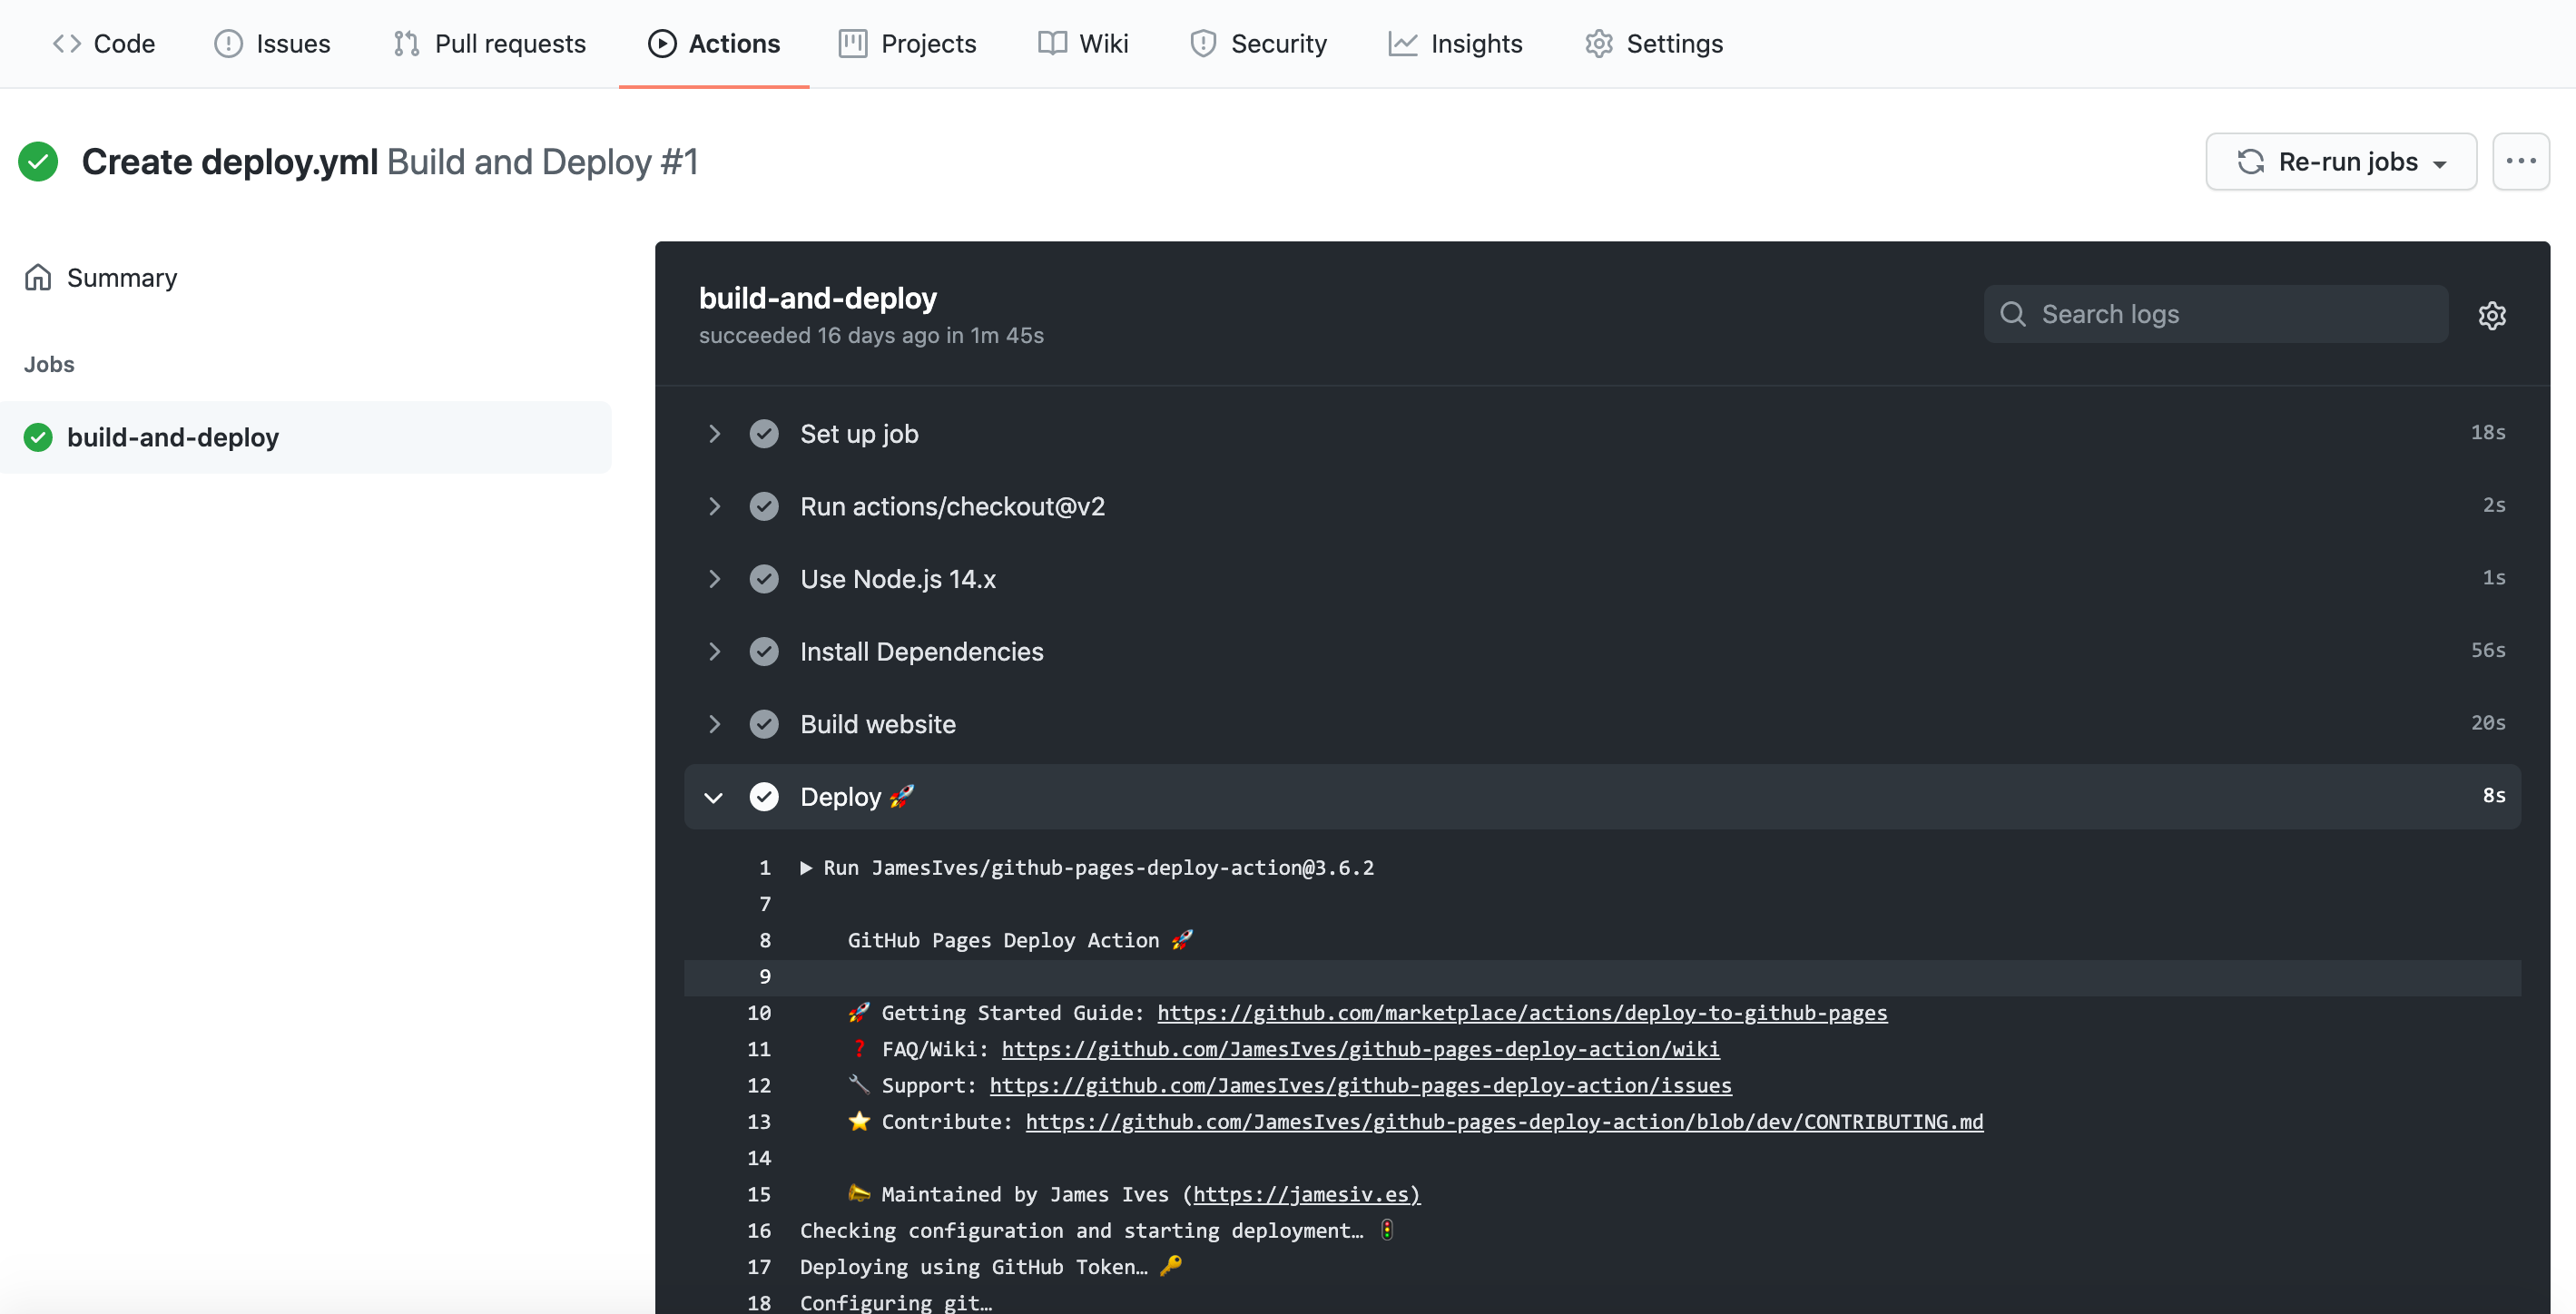
\includegraphics[width=12cm]{gh-actions-log.png}
  \caption{Widok na którym możemy zobaczyć szczegóły danego zadania}
  \label{fig:gh_actions_log}
\end{figure}
Sumarycznie pierwsze budowanie strony zajęło 1min 45sec. Najwięcej czasu zabrało zainstalowanie zależności - aż 56 sekund. Na szczęście GitHub zapewnił akcję, która pozwala cache'ować zależności. Warunkiem koniecznym do działania tego mechanizmu jest posiadanie pliku z informacjami o wersjach zależności jakich używamy. Nie powinno być to problemem, ponieważ większość współczesnych menadżerów zależności generuje taki plik. Implementując cache'owanie, proces automatyzujący będzie tylko instalował zależności, jeżeli jakaś ich wersja się zmieni - w reszcie przypadków proces używa plików z cache'a.
\par
Po tym, gdy pliki z stroną „wylądowały” na gałęzi \textit{gh-pages}, GitHub powinien zakolejkować proces publikacji strony. Jest to rzecz, nad którą nie mamy kontroli.
\begin{figure}[htbp]
  \centering
  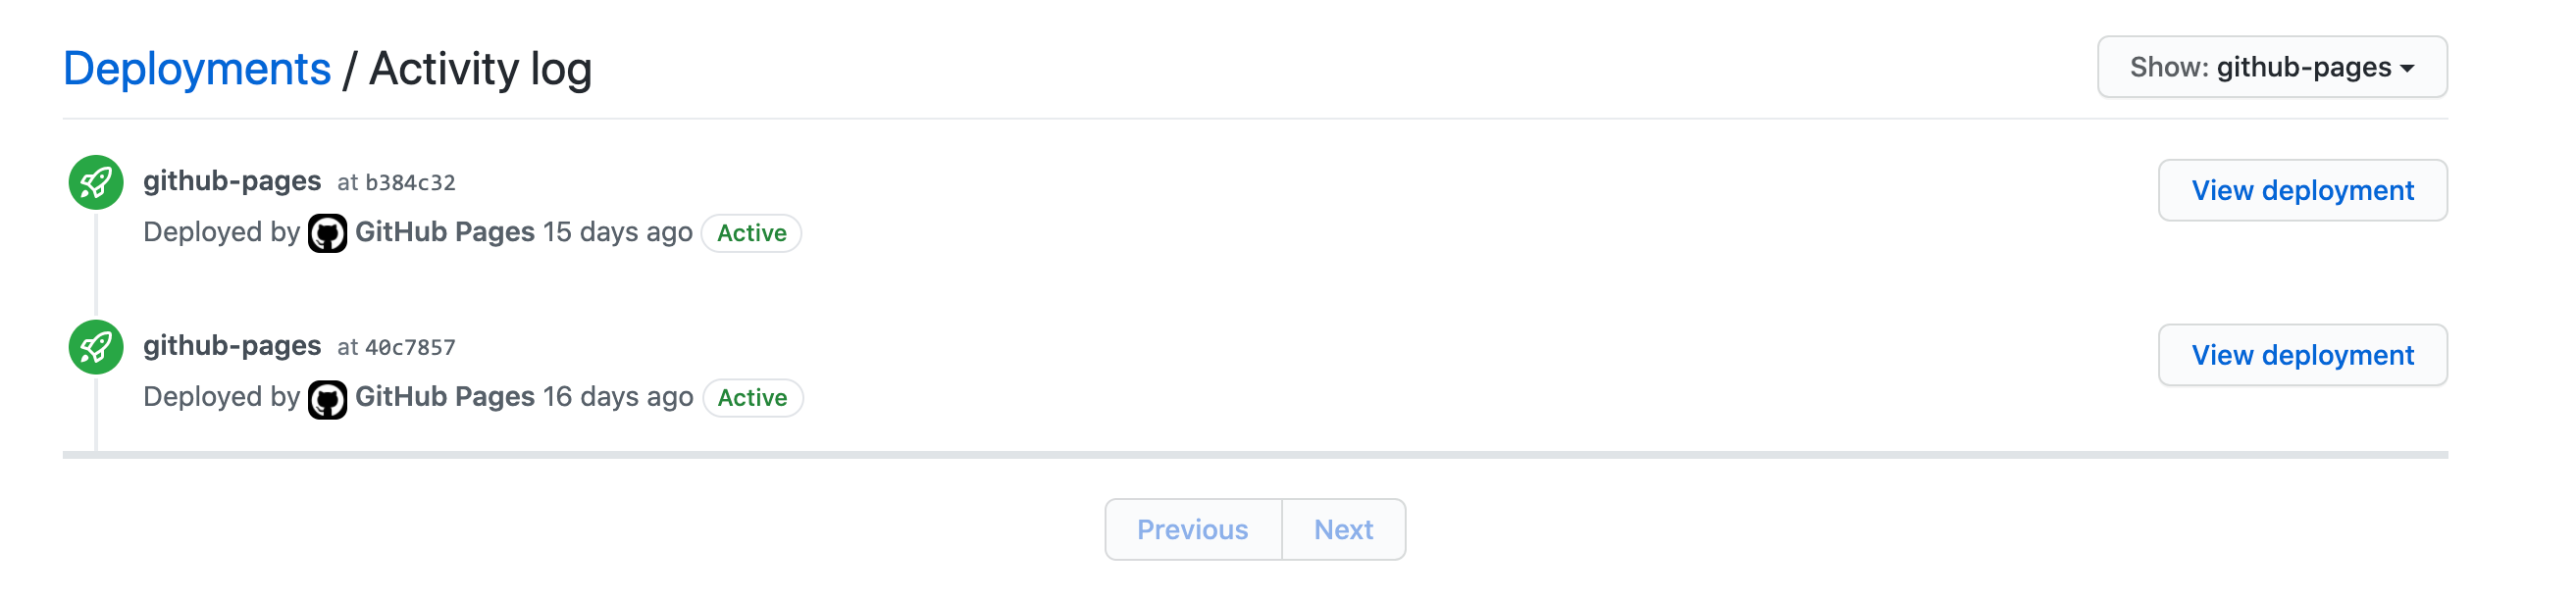
\includegraphics[width=12cm]{gh_pages_deploy.png}
  \caption{Widok z publikacjami strony}
  \label{fig:gh_pages_deploy}
\end{figure}
\par
GitHub wewnętrznie bierze pliki strony z gałęzi, którą ustawiliśmy, i publikuje to na swoich serwerach. Finalnie omawiana strona jest dostępna pod adresem \textit{https://arturkasperek.github.io/static-website-with-ci-cd/}. GitHub pages samo w sobie nie ogranicza nas do używania domeny \textit{github.io}. Jeżeli posiadamy własną domenę, możemy odpowiednio tak przekierować ruch do GitHub'a, że finalny użytkownik nie będzie wiedział, gdzie strona jest hostowana.
\par
Dzięki zapewnieniu modułowości, GitHub Actions może pochwalić się dużą biblioteką akcji stworzoną przez społeczeństwo. Oto lista ciekawych akcji:
\begin{itemize}
  \item jakejarvis/s3-sync-action - jest to akcja, która pozwala synchronizować dany folder repozytorium z folderem na usłudze hostingowej AWS S3. Może być użyteczna, jeżeli chcielibyśmy danej grupie deweloperów dać możliwość wysyłania plików na S3, bez konieczności dawania dostępu do panelu administratora AWS,
  \item repo-sync/github-sync - akcja ta potrafi synchronizować dane repozytorium z innym repozytorium dostępnym w sieci. Jest ona szczególnie użyteczna, gdy pracujemy nad fork'iem (fork to kopia projektu która rozwija się niezależnie względem oryginału) jakiegoś projektu i chcemy utrzymać zgodność z oryginałem. GitHub Actions pozwala na uruchamianie danego procesu automatyzującego automatycznie na podstawie planera. Dzięki temu możemy wykorzystać tą akcję, by co jakiś czas synchronizowała nasze repozytorium z macierzystym projektem,
  \item release-drafter/release-drafter - akcja jest szczególnie użyteczna, jeżeli nasz projekt chce korzystać z dobrych praktyk, dotyczących publikacji oprogramowania. Akcja ta oblicza, jakie zmiany w kodzie nastąpiły od ostatniej publikacji i tworzy wstępną publikację na GitHub'ie z opisem zmian, które dokonaliśmy. Akcja ta jest oparta na commit'ach, dlatego warto by one były dobrze opisane. Jeżeli użyjemy odpowiednich prefixów jak \textit{feature} oraz \textit{bug}, akcja będzie w stanie lepiej sformatować opis publikacji,
  \item zaproxy/action-baseline - jest to akcja, która jest oparta o użycie narzędzia ZAP - to program, który analizuje nasz kod pod względem różnorakich luk bezpieczeństwa. Finalnie jeżeli akcja w wyniku swojego działania znajdzie jakieś podatności to tworzy automatycznie \textit{issue} (system na GitHub'ie, który pozwala śledzić błędy). Jest to ciekawa opcja, jeżeli chcemy jak najbardziej zabezpieczyć się przed ewentualnymi atakami hackerów.
\end{itemize}
Wszystkie powyższe rzeczy moglibyśmy wykonać, używając akcji, która uruchamia skrypt bash'owy. Takie podejście jednak miałoby sporo wad - bylibyśmy zmuszeni spędzić sporo czasu, by wszystko zgrać tak jak chcemy. Dodatkowo prawdopodobnie nie pokrylibyśmy różnych przypadków brzegowych. Dzięki gotowym akcjom czas konfiguracji środowiska do automatyzacji skraca się do minimum, a my możemy się skupić na rozwiązywaniu innych problemów.
\subsection{Program graficzny używający WinAPI - przykład użycia GitLab CI}
Programy z interfejsem graficznym stanowią "lwią" część dostępnych programów dla systemu operacyjnego Windows. Jedną z dróg by tworzyć aplikacje dla Windows'a jest użycie interfejsu programistycznego WinAPI. Sam interfejs WinAPI został zaprojektowany by dobrze działać z językiem programowania C - \cite{WinAPI} aczkolwiek może być on wykorzystywany przez inne języki. Przykładem jest tutaj język C\# który umożliwia tworzenie aplikacji z wykorzystaniem WinAPI. 
\par
Jedną z ważnych rzeczy dla systemu Windows jest komunikacja między poszczególnymi oknami graficznymi. Windows zapewnia nam specjalny interfejs który pozwala wysyłać wiadomości między poszczególnymi oknami. Funkcja która pozwala wysyłać takowe wiadomości nazywa się \textit{SendMessage}. Funkcja ta przyjmuje następujące argumentu:
\begin{itemize}
  \item HWND hWnd - uchwyt do okna które ma otrzymać wiadomość, jeżeli parametr jest równy informację dostaną wszystkie okna wyższego rzędu,
  \item UINT Msg - typ wiadomości którą chcemy wysłać,
  \item WPARAM wParam - dodatkowy obiekt z danymi, zależny od typu wiadomości,
  \item LPARAM lParam - dodatkowy obiekt z danymi, zależny od typu wiadomości.
\end{itemize}
Niektóre Windows'owe programy graficzne za pomocą tej funkcji wysyłają wszelakie logi do aplikacji trzecich. Aplikacje te w ładny sposób prezentują logi. Dzięki takiemu podejściu kod aplikacji głównej jest mniej zawiły ponieważ nie musi on zapewnić interfejsu do wyświetlania takich logów.
\par
Przykładem aplikacji którą używa powyższy wzorzec jest gra komputerowa "Gothic II"©. Jeżeli uruchomimy główny plik .exe z odpowiednim parametrem to wtedy program za pomocą funkcji \textit{SendMessage} zaczyna wysyłać do wyższych okienek wszelakie logi diagnostyczne. Przykładowe wywołanie Gothic2.exe włączające logi:
\begin{lstlisting}[caption={Gra Gothic włącza się w trybie okienkowym, bez muzyki i dźwięków oraz z wysyłaniem logów}]
  Gothic2.exe -zwindow -znomusic -znosound -zlog:5,s
\end{lstlisting}
Twórcy dostarczyli także aplikację, która nasłuchuje logi wysyłane przez grę - jej nazwa to zSpy.
\begin{figure}[htbp]
  \centering
  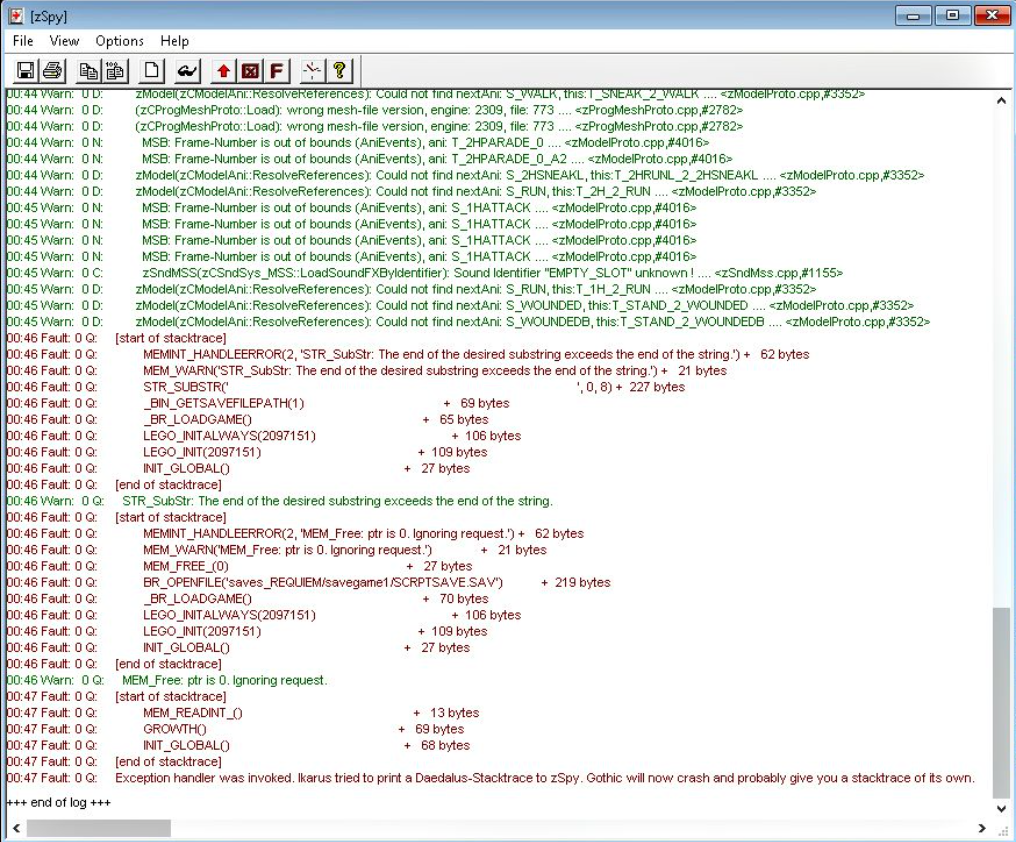
\includegraphics[width=10cm]{zspy.png}
  \caption{zSpy - aplikacji do wyświetlania logów gry Gothic}
  \label{fig:gh_pages}
\end{figure}
\par
Załóżmy, że posiadamy aplikację okienkową do liczenia liczb pierwszych, która za pomocą graficznego interfejsu pozwala wyliczyć liczby pierwsze do podanej maksymalnej liczby. Cechy tej aplikacji to:
\begin{itemize}
  \item Jest napisana w języku C++,
  \item Wykorzystuje sito Eratostenesa by wyliczyć liczby pierwsze dla podanego maksimum,
  \item Wysyła logi w formacie JSON za pomocą funkcji \textit{SendMessage},
  \item Jeżeli uruchomimy tę aplikację z poziomu wiersza poleceń i podamy parametr liczbowy to zainicjalizujemy program bez potrzeby podawania z pomocą interfejsu graficznego liczby maksymalnej.
\end{itemize}
Chcielibyśmy umożliwić uruchomienie tego programu na środowisku serwerowym, które nie posiada kontekstu graficznego. Dodatkowo chcielibyśmy to zrealizować za pomocą platformy GitLab CI która umożliwia uruchomienie danego potoku automatyzującego z parametrem dostarczonym przez użytkownika. Dzięki takiej konfiguracji bez konieczności uruchamiania systemu Windows zyskalibyśmy możliwość uruchamiania algorytmu, który jest zaimplementowany w aplikacji graficznej.
\par
Sam interfejs graficzny aplikacji jest bardzo prosty. Składa się on z pola tekstowego gdzie użytkownik podaje liczbę, przycisku który uruchamia algorytm oraz pola tekstowego gdzie wyświetlany jest wynik.
\begin{figure}[htbp]
  \centering
  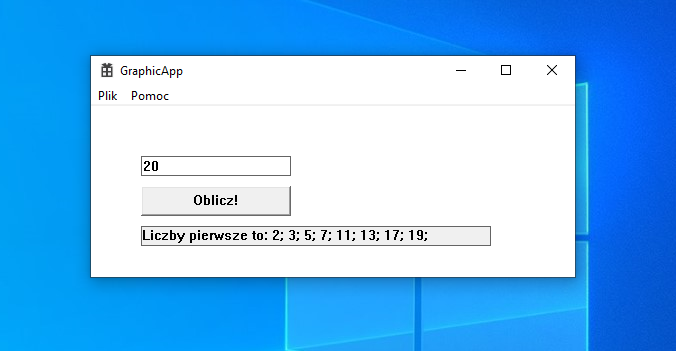
\includegraphics[width=10cm]{graphic-app-preview.png}
  \caption{Aplikacja do wyznaczania liczb pierwszych uruchomiona na Windows 10}
  \label{fig:gh_pages}
\end{figure}
\par
Teraz chcielibyśmy uruchomić naszą aplikację na środowisku serwerowym. W przypadku GitLab'a mamy dostęp do maszyn na których działa tylko Linux. Jest to pierwszy problem który musimy rozwiązać - nie jest możliwe uruchomienie natywnie aplikacji stworzonej dla Windowsa na Linuxie. W tym aspekcie może nam pomóc projekt \textit{Wine}. Nazwa jest akronimem rekurencyjnym, z ang. \textit{Wine is not an emulator}. Akronim ten przypomina nam, że wine nie powinien być postrzegany jako emulator Windows'a. Wine jest dodatkową warstwą, która tłumaczy wywołania systemowe specyficzne dla Windowsa na te zrozumiałe dla Linuxa. By nie marnować czasu na instalację wine, użyjemy gotowego obrazu docker'owego, który ma już zainstalowanego wine z wszelakimi zależnościami. Obraz ten możemy pobrać za pomocą komendy:
\begin{lstlisting}[caption={Pobierania obrazu który ma zainstalowane środowisko wine}]
  docker pull scottyhardy/docker-wine
\end{lstlisting}
Cechą tego obrazu jest fakt, że w prosty sposób możemy uruchomić w kontenerze serwer RDP (protokół pulpitu zdalnego), który pozwoli połączyć się z kontenerem w sposób graficzny. Jest to przydatne do debugowania. Gdy już uruchomimy ten obraz z odpowiednimi parametrami startowymi możemy przetestować jak nasza aplikacja działa na systemie Linux. Załóżmy, że chcielibyśmy zobaczyć liczby pierwsze nie większe niż 14. W tym celu musimy wykorzystać komendę \textit{wine GraphicApp.exe 14} i poczekać aż wine się zainicjalizuje. Dzieje się to wtedy kiedy komenda \textit{wine} jest użyta po raz pierwszy.
\begin{figure}[htbp]
  \centering
  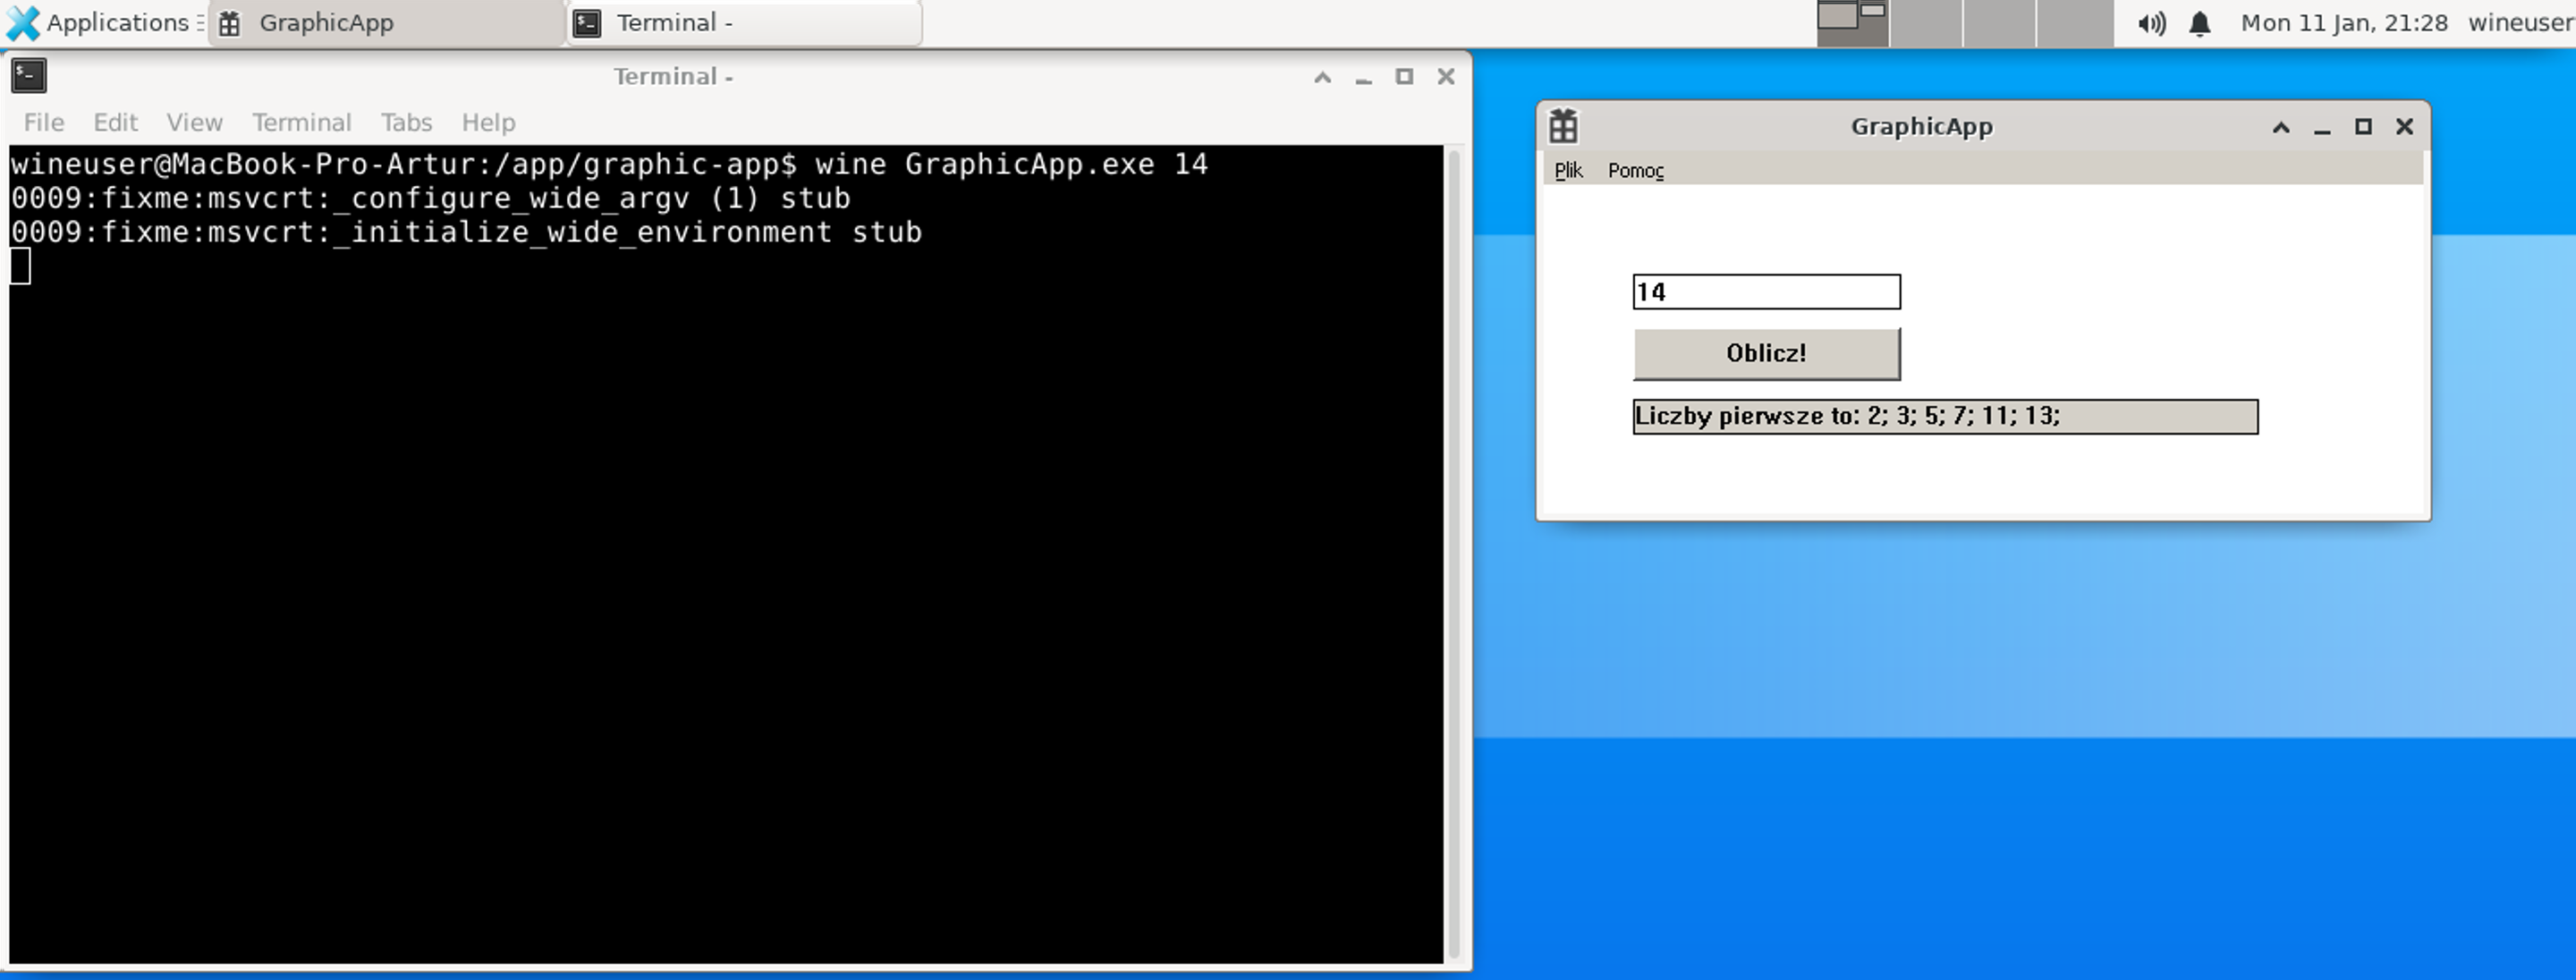
\includegraphics[width=13cm]{wine-docker.png}
  \caption{Aplikacja graficzna uruchomiona na systemie Linux}
  \label{fig:wine_docker}
\end{figure}
Po chwili powinniśmy zauważyć okienko w którym powinien być wynik dla podanej liczby maksymalnej.
\par
Teraz gdy już jesteśmy w stanie uruchomić nasz program na systemie Linux musimy w jakiś sposób stworzyć interfejs który pozwoli nam wysyłać logi do zewnętrznej aplikacji. Chcielibyśmy by nasza aplikacja do wyświetlania logów była stworzona za pomocą technologii NodeJS. Sam obraz \textit{scottyhardy/docker-wine} nie zawiera środowiska NodeJS. Najrozsądniejszym wyjściem jest użycie dedykowanego obrazu dla NodeJS - dzięki temu zyskujemy większą separację między tymi dwoma światami. By aplikacja w innym kontenerze miała dostęp do logów, które są wysyłane w wine musimy stworzyć pośrednią aplikację. Jej celem będzie nasłuchiwanie zdarzeń okienkowych oraz wysyłanie logów dalej za pomocą web socketów. 
\par
Główną częścią pośrednika jest nasłuchiwanie na zdarzenia okienkowe. Jest za to odpowiedzialny poniższy kod:
\begin{lstlisting}[caption={Fragment aplikacji odpowiedzialnej za dalsze przekazywanie logów}]
  LRESULT CALLBACK WindowProcedure (HWND hwnd, UINT message, WPARAM wParam, LPARAM lParam)
  {
      switch (message)                  /* handle the messages */
      {
          case WM_COPYDATA:
              {
                  COPYDATASTRUCT* pcds = (COPYDATASTRUCT*)lParam;
                  char * lpszString = (char *)(pcds->lpData);

                  printf("Web Broadcaster received COPYDATA message!!\n");
                  sendMessage((char*)lpszString);
                  break;
              }
          case WM_DESTROY:
              PostQuitMessage (0);       /* send a WM_QUIT to the message queue */
              break;
          default:                      /* for messages that we don't deal with */
              return DefWindowProc (hwnd, message, wParam, lParam);
      }

      return 0;
  }
\end{lstlisting}
Jeżeli typ wiadomości otrzymany przez aplikacje jest równy \textit{WM\_COPYDATA} to w takim wypadku treść wiadomości jest wysyłana dalej do serwera, z którym pośrednik jest połączony.
\par
Tworząc aplikację opartą na WebSocket'ach należy mieć na względzie to, że musimy stworzyć serwer, który będzie miejscem gdzie logi będą parsowane i w ładny sposób drukowane na standardowym wyjściu. Kod serwera jest stworzony w języku JavaScript i wygląda następująco:
\begin{lstlisting}[caption={Kod aplikacji serwera który wyświetla logi z aplikacji graficznej}]
var net = require('net');

try {
  let activeSockets = [];
  let graphicAppSendResult = false;
  let connectionCounter = 0;
  var server = net.createServer(function(socket) {
    socket.pipe(socket);
    activeSockets.push(socket);
    connectionCounter++;
    socket.on('data', function(data) {
      const dataString = (data.toString() || '');
      const parsed = dataString.match(/{(.*?)}/gm);

      if ( parsed ) {
        parsed.forEach(item => {
          try {
            const result = JSON.parse(item);

            if ( result.log ) {
              console.log(`Log: ${result.log}`);
            } else if (result.result) {
              console.log(`Result: ${result.result}`);
            } else {
              console.log(`Other unknown: ${result}`);
            }
          } catch (e) {
            console.error('Problem with parsing', item);
          }
        });
        activeSockets.forEach(i => i.write('graphic-app-finished-calc'));
        graphicAppSendResult = true;
      } else {
        console.log('Not known input data', dataString)
      }
    });

    socket.on('close', function () {
      console.log('Closing socket');
      const toRemove = activeSockets.find(i => i === socket);
      activeSockets = activeSockets.filter(i => i !== toRemove);
    });
    socket.on('error', function (e) {
      console.log('Socket error', e);
    });

    if ( connectionCounter >= 2 ) {
      activeSockets.forEach(i => i.write('broadcaster-connected'));
    }
    if (graphicAppSendResult) {
      socket.write('graphic-app-finished-calc');
    }
  });
  server.listen(8080, () => {
    console.log('Web listener waiting on 8080');
  });
} catch (e) {
  console.log('Web listener error', e);
  throw e;
}
\end{lstlisting}
Jeżeli spojrzymy na linię 13 powyższego listingu to zauważymy kod odpowiedzialny za odbieranie wiadomości z WebSocket'a. Należy mieć na względzie, że protokół WebSocket nie gwarantuje nam, że wiadomość odebrana na serwerze będzie pojedynczą wiadomości wysłaną przez klienta. Może się zdarzyć sytuacja w której dwie wiadomości będą złączone ze sobą. W tym celu w linijce 15 za pomocą wyrażenia regularnego szukamy wiadomości, które spełniają wzorzec formatu z aplikacji graficznej. Kolejne linijki parsują otrzymaną wiadomość oraz wyświetlają ją na ekranie. W linijce 34 informujemy klientów podłączonych do serwera, że aplikacja graficzna skończyła obliczenia. Wysyłając tę wiadomość dajemy znać, że aplikacja graficzna skończyła swoje obliczenia i proces na serwerze może być już zamknięty.
\par
Całość projektu uzupełniają dwie mini aplikacje w NodeJS. Celem pierwszej jest czekanie aż aplikacja graficzna będzie już aktywna. Celem drugiej jest czekanie aż pośrednik który przekazuje wiadomości z środowiska WinAPI do WebSocket'ów połączy się z serwerem. Bez tych aplikacji nie możliwa byłaby kontrola procesu uruchomionego na serwerze.
\par
Finalnie uruchomienie programu sprowadza się do odpowiedniego uruchamiania różnych poleceń docker'owych:
\begin{lstlisting}[caption={.gitlab-ci.yml - konfiguracji procesu automatyzującego}]
run-calculation:
  image: docker:latest
  stage: build
  services:
    - docker:dind
  script:
    - env
    - echo "Creating docker network"
    - docker network create graphic-app-network
    - echo "Running web listener"
    - docker run -d -v $(pwd):/app --network graphic-app-network --name web-listener node:14-alpine node /app/web-listener/main.js
    - echo "Running wine container"
    - docker run -d -it -v $(pwd):/app --rm --hostname="$(hostname)" --network graphic-app-network  --publish="3389:3389/tcp" --name docker-wine-container scottyhardy/docker-wine tail -f /dev/null
    - sleep 3
    - echo "Running broadcaster"
    - docker exec -d docker-wine-container /bin/bash -c "/app/start.sh"
    - echo "Waiting for broadcaster to be up"
    - docker ps
    - docker logs web-listener
    - docker run -v $(pwd):/app --network graphic-app-network node:14-alpine node /app/wait-for-broadcaster/main.js
    - echo "Running graphic app"
    - docker exec -d docker-wine-container /bin/bash -c "DISPLAY=:1 wine /app/graphic-app/GraphicApp.exe ${PRIME_NUMBERS_LIMIT:-30}" &
    - echo "Waiting for graphic app to finish work"
    - docker ps
    - docker logs web-listener
    - docker run -v $(pwd):/app --network graphic-app-network node:14-alpine node /app/wait-for-graphic-app/main.js || echo "Failed to wait for graphic..."
    - docker logs web-listener
  only:
    - master
\end{lstlisting}
Powyższy plik to plik konfiguracyjny GitLab CI. Zawiera on informację o potokach które nasze środowisko ma zawierać. W naszym przypadku mamy tylko jeden potok \textit{run-calculation} który jest odpowiedzialny za uruchomienie aplikacji graficznej. Proszę zwrócić, że w linijce 22 uruchamiamy aplikację graficzną. Dzięki użyciu tutaj parametru środowiskowego \textit{PRIME\_NUMBERS\_LIMIT} zyskujemy możliwość późniejszego uruchomienia potoku z dowolną wartością liczbową. Dzięki temu użytkownik będzie mógł zobaczyć działanie programu dla różnych danych wejściowych.
\par
Teraz powinniśmy mieć możliwość włączenia programu z dowolnym parametrem startowym.
\begin{figure}[htbp]
  \centering
  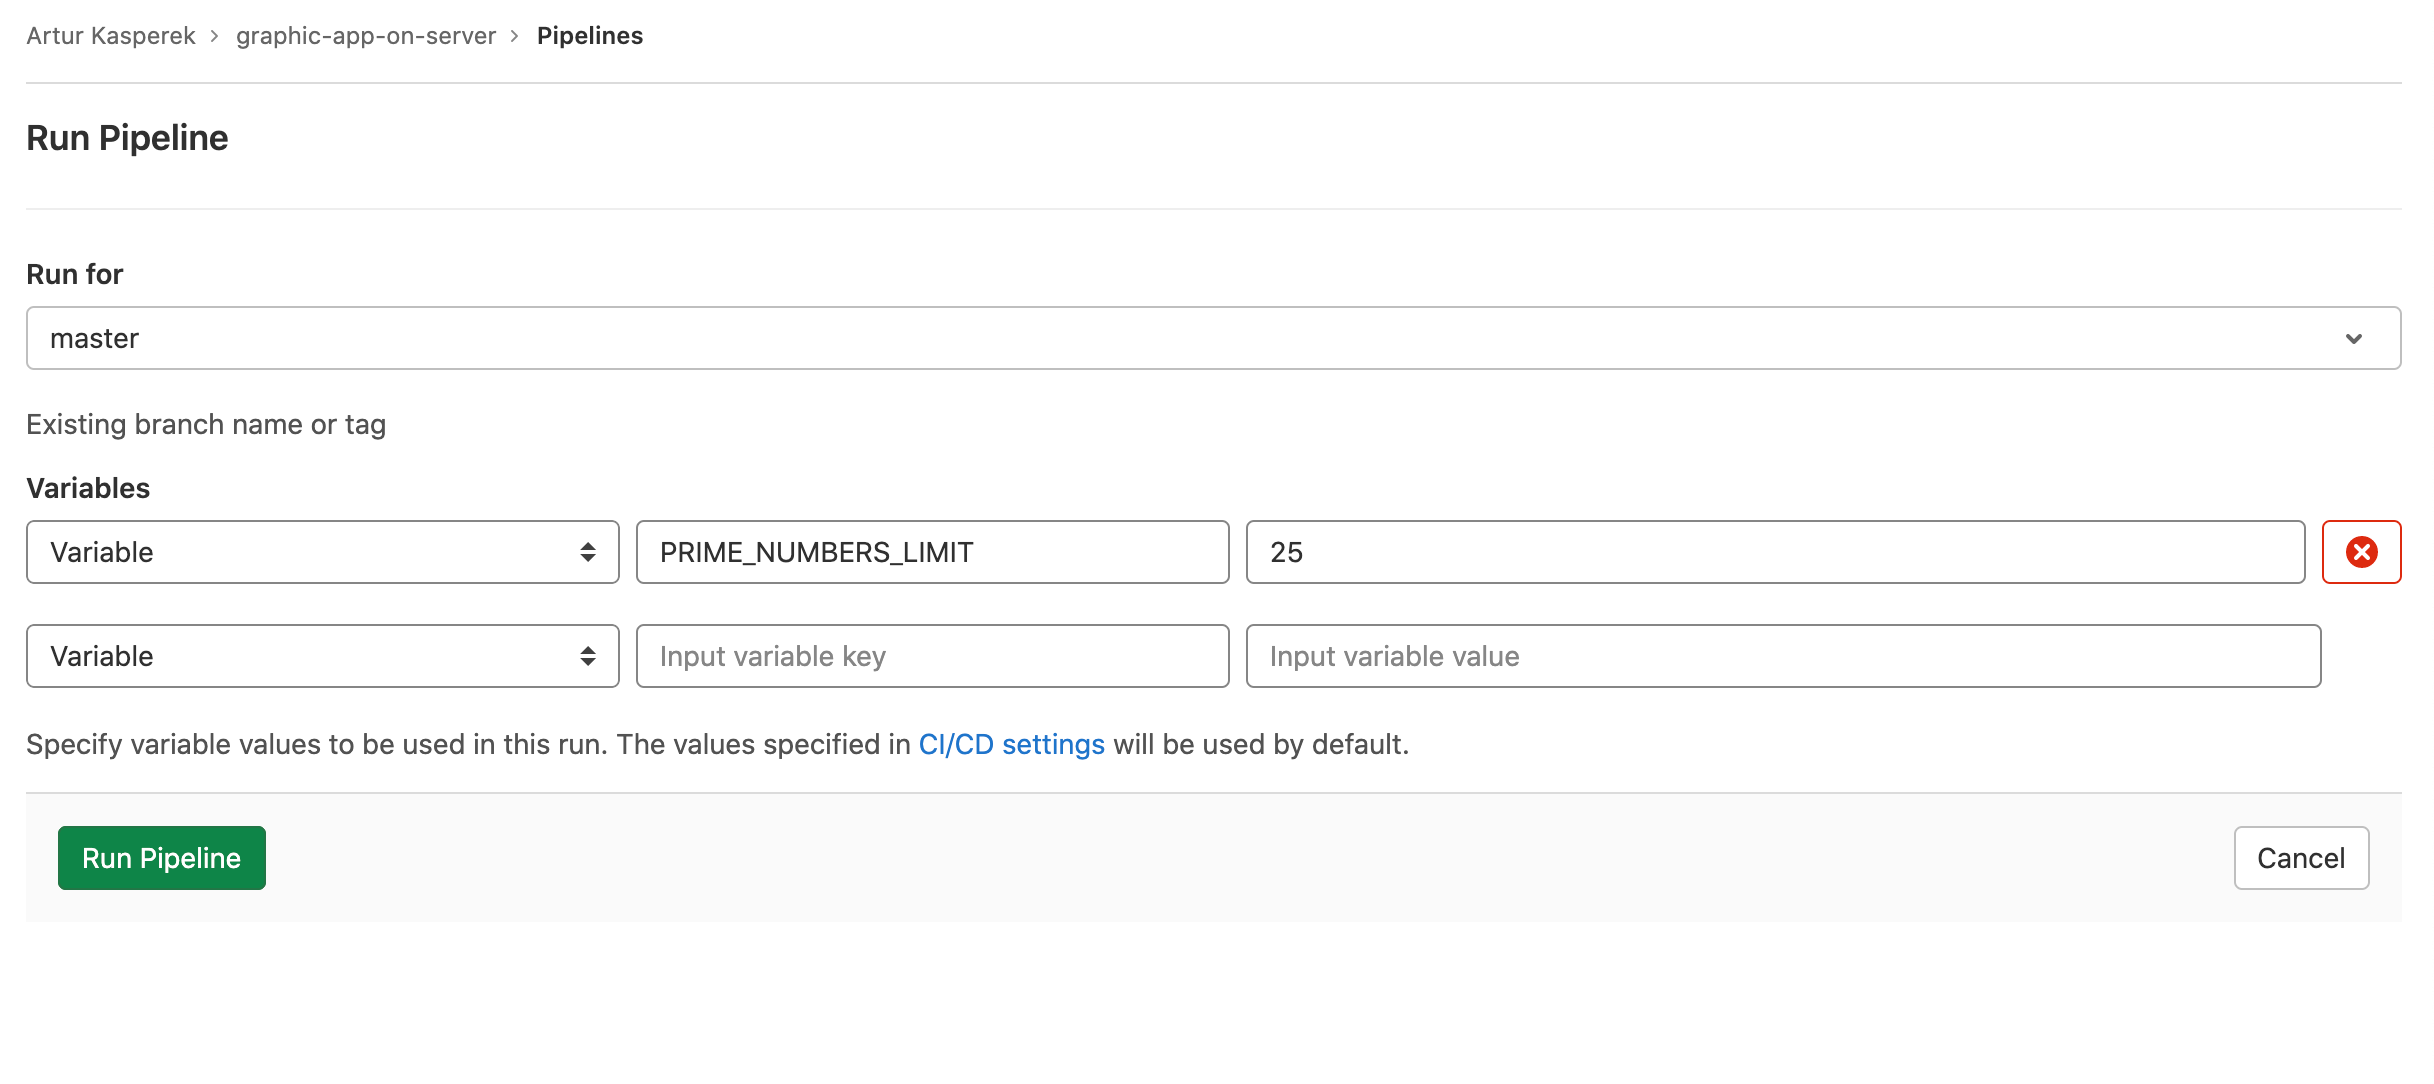
\includegraphics[width=13cm]{gitlab-pipeline.png}
  \caption{Interfejs uruchamiania pipeline'a z zdefiniowanymi parametrami środowiskowymi}
  \label{fig:gitlab_pipeline}
\end{figure}
Po uruchomieniu danego pipeline'u powinniśmy być w stanie przejrzeć logi, które zostały wypisane na standardowe wyjście. W logach tych powinniśmy dostrzec na końcu wiadomości wysłane z aplikacji graficznej. Dzięki temu jesteśmy w stanie stwierdzić jaki jest wynik działania programu graficznego.
\begin{figure}[htbp]
  \centering
  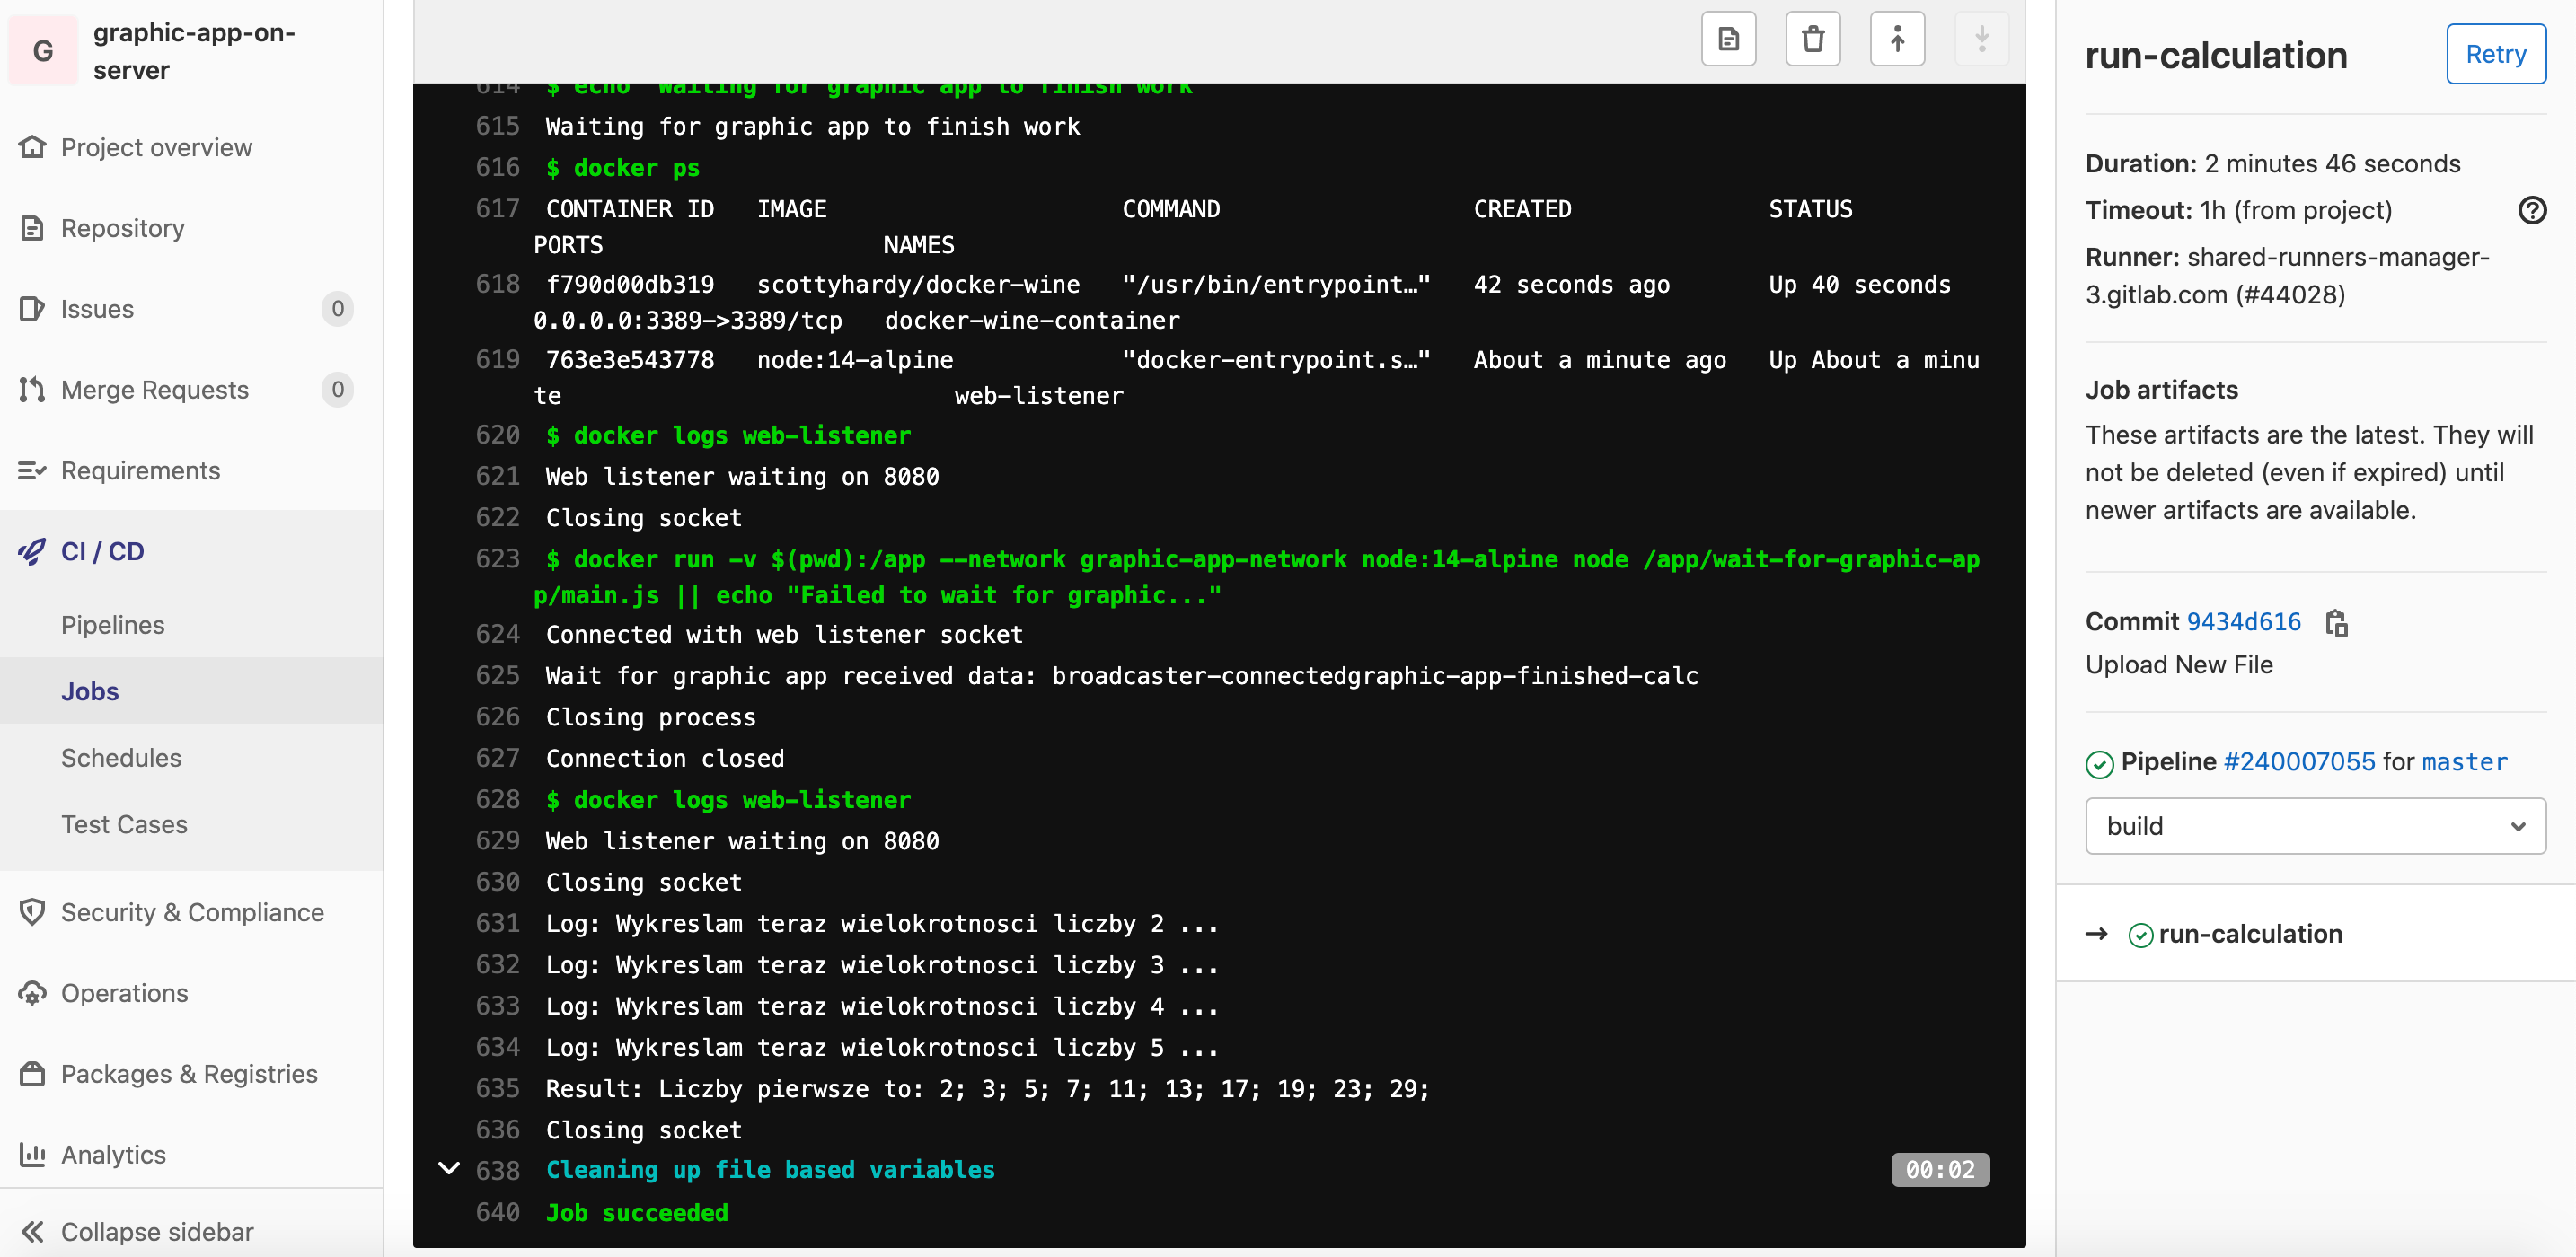
\includegraphics[width=14cm]{gitlab-ci-result.png}
  \caption{Wyniki pipeline'u dla \textit{PRIME\_NUMBERS\_LIMIT} równego 30}
  \label{fig:gitlab_pipeline_result}
\end{figure}
\section{Testy a continuous integration}
W celu lepszego zrozumienia istoty automatyzacji testów konieczne jest najpierw zrozumienie testów samych w sobie. Jak zostało to opisane w rozdziale 1.4 - pisanie testów jest integralną częścią pracy każdego programisty. Wiele osób uważało to dawniej za żmudne zadanie, nieprzynoszące wymiernych korzyści, jednakże z biegiem czasu stało się jasne, że w dużych projektach informatycznych są one konieczne, co widać w dzisiejszych czasach w wypowiedziach wielu osób \cite{UnitOpinions} \cite{UnitResults}.

\subsection{Testy jednostkowe}
Testem jednostkowym nazywa się kod, który jest w stanie wywołać inny fragment kodu programu, a następnie sprawdzić czy działanie tamtego kodu jest zgodne z zakładanym przez programistę działaniem \cite{UnitDefinition}.
\par Autor tej definicji zdefiniował też kilka warunków, które powinien spełniać każdy test jednostkowy dobrej jakości: 
\begin{itemize}
    \item jest w pełni zautomatyzowany - nie wymaga żadnej interakcji od użytkownika,
    \item odizolowany od reszty kodu, którego nie sprawdza oraz od innych testów - w celu spełnienia tego warunku często będą wykorzystywane tak zwane "mocki" oraz "stuby",
    \item nie ma dostępu do baz danych lub plików na dysku,
    \item jest deterministyczny, nie zawiera losowych danych, przy każdym uruchomieniu kodu zwraca taki sam rezultat,
    \item jest szybki - należy pamiętać, że testów będzie w kodzie dużo, a także będą one często uruchamiane,
    \item skupia się na pojedynczym logicznym elemencie programu,
    \item czytelny,
    \item łatwy w zrozumieniu,
    \item wiarygodny - wynika to z dwóch powyższych warunków. Po otrzymaniu wyniku testów nie powinniśmy mieć wątpliwości czy jest on poprawny.
\end{itemize}
Fragmentem kodu, który podlega testom jest zwykle najmniejsza jego część, która odpowiada za jedno logiczne działanie. Najczęściej będzie to więc pojedyncza metoda klasy lub cała klasa. 

Odpowiednie przygotowanie testów jest kluczowe jeśli chcemy uniknąć w naszym projekcie regresji - pojawienia się błędów w kodzie, który wcześniej działał poprawnie ( wiąże się to także z innym rodzajem testów - testami regresyjnymi, których zadaniem jest sprawdzanie, czy wprowadzona zmiana w danym miejscu programu nie spowoduje powstania błędów w innych jego miejscach \cite{RegressionTesting}). 

Warto wspomnieć także o testowaniu tak zwanych przypadków brzegowych (Edge cases). W przypadku gdy w kodzie występuje przykładowo porównanie x$>$5, warto sprawdzić jak dana metoda zachowa się z wartościami 4, 5 oraz 6. Innymi warunkami brzegowymi mogą często być (w przypadku gdy typ danych to integer): 
\begin{itemize}
    \item wartość 0,
    \item wartość ujemna, często -1,
    \item minimalna wartość przewidziana dla funkcji,
    \item maksymalna wartość przewidziana dla funkcji,
    \item wartość odpowiednio mniejsza i większa od wartości minimalnej i maksymalnej, która powinna spowodować błąd.
\end{itemize}

\subsubsection{Wykorzystanie atrap}
Jak zostało to opisane wcześniej - każdy test jednostkowy powinien być odizolowany od reszty kodu i innych zależności zewnętrznych. Należy to rozumieć poprzez bycie odizolowanym od plików na dysku, danych z internetu, dostępu do baz danych wykorzystywanych w projekcie oraz do klas i interfejsów niebędących przedmiotem testów. Konieczność taka zachodzi z kilku powodów, między innymi: 
\begin{itemize}
    \item test może dać nam zły rezultat, nawet gdy sam fragment, który ma on testować nie zawiera żadnych błędów. Błędy wynikają wtedy z innych zależności, które powinny zostać wykryte przez testy przygotowane specjalnie dla nich,
    \item mogą one zajmować zbyt dużo czasu. Szczególnie chodzi tutaj o dostęp do plików na dysku oraz zapytania do bazy danych, które zwykle same w sobie zajmują wielokrotnie więcej czasu niż sam testowany przez nas kod.
\end{itemize}

Oczywistym jest, że nawet gdy sam test nie ma mieć dostępu do zależności zewnętrznych, to sam kod musi ten dostęp posiadać w celu prawidłowego działania. Aby móc poprawnie przetestować taki kod, który wymaga różnych zależności zewnętrznych wykorzystujemy atrapy. Wykorzystywane są one wyłącznie przez testy, nie mają żadnego wpływu na działanie programu. Ich zadaniem jest symulowanie działania prawdziwego kodu, który nie podlega naszym testom. W praktyce najczęściej wykorzystywany będzie do tego specjalny framework, np. Moq dla C\#, Mockito dla Java lub unittest.mock dla pythona. 

W literaturze wyznaczonych zostało wiele rodzajów atrap. Znaczna część dostępnych frameworków nie rozdziela ich jednak, a duża część społeczności różnie definiuje poszczególne rodzaje. Warto wymienić kilka najpopularniejszych używanych określeń: 
\begin{itemize}
    \item Stub - najprostszy rodzaj atrapy. Potrafi ona przechowywać dane predefiniowane jej w trakcie pisania testu oraz odpowiedzieć tymi danymi podczas wywołania go. Nadaje się idealnie do symulowania działania bazy danych, która ma zwrócić wartość na podstawie zapytania,
    \item Mock - są to obiekty, które mają możliwość otrzymywania danych oraz weryfikowania, czy są one zgodne z oczekiwaniami w danym teście,
    \item Fake - bardziej zaawansowane rodzaje atrap. Posiadają one faktyczne implementacje kodu, zwykle pisane jednak specjalnie pod dany przypadek testowy. Kod ten jest znacznie mniej rozbudowany od produkcyjnego, pozwala jedynie na przetestowanie wymaganej funkcjonalności. 
\end{itemize}

\subsubsection{Przykładowy test jednostkowy}
Do napisania najprostszego testu jednostkowego w języku python nie jest konieczne nawet wykorzystanie żadnego zewnętrznego frameworka. 

\begin{lstlisting}[caption={Test jednostkowy w języku Python}]
string = "asda"

assert isinstance(string, str), "Not string"
assert len(string) > 0, "No text to capitalize"

x = string.upper()
\end{lstlisting}

Wykorzystana została tutaj asercja, która jest podstawą każdego testu jednostkowego. Jej zadaniem jest sprawdzenie czy dana zależność określona w kodzie przez programistę jest spełniona. W tym przypadku wykorzystane zostały dwie asercje. Możliwe jest zrezygnowanie z pierwszej, ponieważ sprawdza ona czy obiekt jest typu string, co zostałoby wykryte później przez funkcję upper(). Istotniejsza jest druga z nich, która sprawdza czy dany string nie jest pusty. Jest to o tyle istotne, że funkcja upper() przyjmuje puste stringi i nie zwróci nam dla nich żadnego błędu. Wykorzystanie takiej asercji powoduje, że programista może w dalszej części kodu zakładać, że wartość, którą otrzyma z funkcji upper() nie będzie pusta. W przypadku użycia pustego łańcucha znaków otrzymamy następujący komunikat: 

\begin{lstlisting}[caption={Błąd asercji podczas testu}]
AssertionError                            Traceback (most recent call last)
<ipython-input-40-7526aaf9a6e8> in <module>
      2 
      3 assert isinstance(string, str), "Not string"
----> 4 assert len(string) > 0, "No text to capitalize"
      5 
      6 x = string.upper()

AssertionError: No text to capitalize
\end{lstlisting}

Użycie dowolnego niepustego łańcucha znaków spowoduje, że test jednostkowy zostanie pomyślnie wykonany i nie zostanie zwrócony żaden błąd. 

\begin{figure}[htbp]
    \centering
    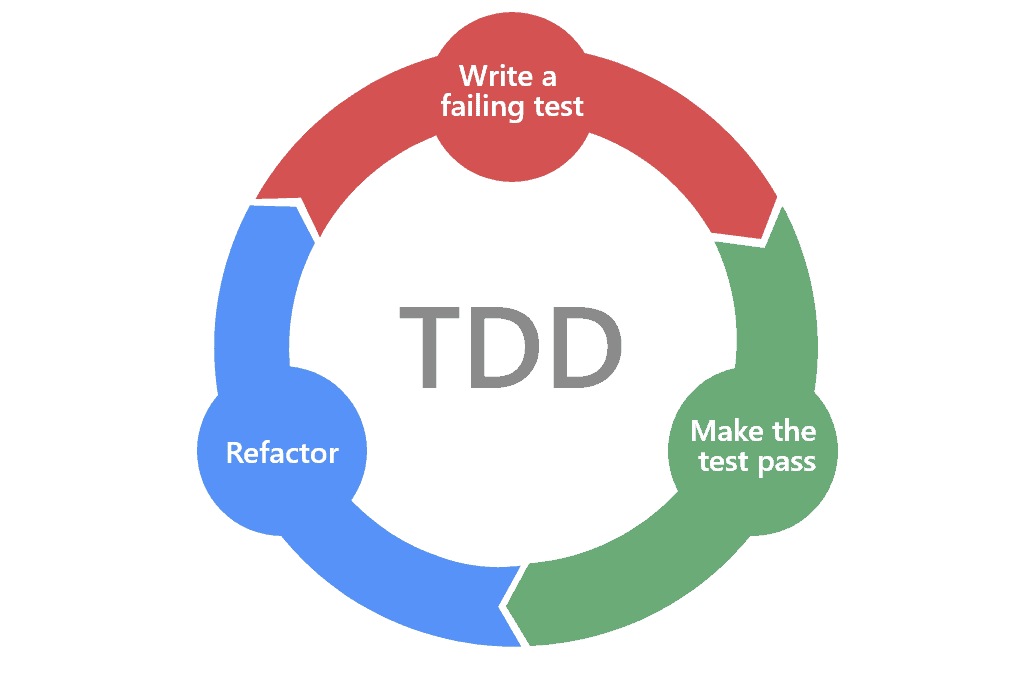
\includegraphics[width=10cm]{images/tdd.png}
    \caption{Zasada Red-Green-Refactor}
    \label{fig:redgreen}
\end{figure}

\subsubsection{Metodyki pisania testów}
\par Najpopularniejsze obecnie są dwie metody pisania testów: 
\begin{itemize}
    \item TDD - Test Driven Development - zaproponowana została przez Kenta Becka w 2002 roku \cite{TestDrivenDevelopment}. Zakłada, że testy będą napędzały tworzenie projektu i stały u jego podstawy. 
    \par Pierwszym krokiem przy implementacji nowej funkcji w naszym projekcie powinno być napisanie samego testu, który oczywiście na początku nie powiedzie się, ponieważ kod, który ma on testować nie został jeszcze napisany. Po napisaniu testu przechodzi się do pisania kodu, który w jak najłatwiejszy sposób będzie w stanie zaliczyć napisany przez nas test. Ostatnim krokiem tego cyklu jest refactoring kodu, polepszający jego jakość samą w sobie, ale bez zmieniania jego funkcjonalności, tak aby spełniał on oczekiwane standardy.
    Takie podejście pozwala na tworzenie dobrze zaprojektowanego kodu, który jest w całości pokryty testami, co owocuje w przyszłości, kiedy konieczne jest wprowadzanie zmian w bazie kodu.
    
    Pozwala to również na wymuszenie na osobach piszących kod, aby był on dobrze przemyślany. Konieczność napisania testu przed implementacją funkcjonalności wymusza na programiście, aby zastanowił się dogłębniej jak ma wyglądać struktura jego kodu oraz co chce on osiągnąć implementując daną klasę. 
    
    Podejście TDD zapewnia więc wiele zalet, ale nie jest ono oczywiście całkowicie pozbawione wad. Jedną z nich jest konieczność nauczenia programistów tej metodologii w przypadku jeśli wcześniej nie mieli z nią do czynienia. Główną wadą jest jednak znacznie zwiększony narzut czasowy na pisanie testów wynikający z wykorzystania TDD. Duże pokrycie kodu testami zajmuje programistom zwykle znacznie więcej czasu niż podczas standardowego implementowania funkcjonalności, a następnie napisania testów dla wybranych wedle uznania fragmentów kodu. Zainwestowany jednak w ten sposób czas zwraca się w późniejszych fazach projektu, jeśli okazuje się, że konieczna jest jakaś zmiana w strukturze kodu. Najwięcej czasu oszczędza się w porównaniu do standardowych metod pisania kodu na poprawianiu błędów działania programu. Wszystkie błędy poprawiane są na bieżąco, nie ma możliwości implementacji funkcjonalności bez poprawnego spełnienia napisanego wcześniej testu. W przypadku gdy taki test nie został nigdy napisany lub gdy błąd danej funkcji wynika z innego fragmentu kodu, jego znalezienie i naprawa może pochłonąć dużo czasu pracy programisty. 
    
    \item BDD - Behavior Driven Development - metodologia zaproponowana przez Dana Northa w 2006 roku \cite{BehaviourDrivenDevelopment}. Zakłada ona zaangażowanie w tworzenie oprogramowania osób nietechnicznych - analityków oraz klientów dla których oprogramowanie jest tworzone. Pozwala to na lepsze określenie kierunku, w którym zmierza rozwój aplikacji oraz pozwala na uniknięcie nieporozumień dotyczących projektu pomiędzy programistami, a osobami, które mają być odbiorcami programu. 
    \par Pierwszym krokiem przy tworzeniu nowej funkcjonalności jest zdefiniowanie przez zespół biorący udział w tworzeniu programu tak zwanych "User Stories". 
    Tworzone są one według zasady "Given - When - Then (Zakładając - Gdy - Wtedy)". Można w ten sposób łatwo opisać testy, które każdy będzie w stanie zrozumieć, a następnie zaimplementować przy użyciu odpowiedniego frameworka, np. JBehave dla Java lub Behave dla Pythona. 
    
    \begin{lstlisting}[caption={Przykładowe User Story}]
User Story: Spend points in game

As a game user
In order to get a spell
I want to spend my spell points

Given that I have 5 spell points available
When I spend 2 spell points on a spell
Then I should have 3 spell points and a new spell

    \end{lstlisting}
\end{itemize}

\subsection{Testy integracyjne}
Podczas omawiania testów jednostkowych duża uwaga została nałożona na konieczność odizolowania takiego testu od reszty kodu oraz innych zależności zewnętrznych. Testy integracyjne z kolei skupiają się właśnie na sprawdzeniu czy nasz kod działa poprawnie z innymi jego fragmentami oraz zależnościami zewnętrznymi, takimi jak komunikacja z bazami danych, API działającym na serwerze lub plikami na dysku. 

Głównym wyzwaniem przy pracy z testami integracyjnymi jest zwykle znalezienie przyczyny problemu, przez który testy nie mogą się powieść. W testach jednostkowych - o ile były poprawnie napisane nie stanowi to zwykle dużego problemu, z kolei testując więcej elementów znalezienie przyczyny problemu może wymagać więcej wysiłku. Problem może wynikać między innymi z implementacji danych systemów przez różne osoby w różnym czasie, kiedy mogły zmienić się wymagania i oczekiwania od projektu.

Należy pamiętać, że testy integracyjne trwają znacznie dłużej niż jednostkowe, z reguły będzie ich także znacznie mniej, z uwagi na to, że takich zależności będzie mniej niż najmniejszych możliwych do przetestowania fragmentów kodu. Z tego powodu warto rozważyć w projekcie zmianę strategii testowania w porównaniu z testami jednostkowymi. Tamte można zwykle wykonywać zarówno przy każdej kompilacji programu oraz przy publikowaniu zmian w repozytorium kodu. Przy testach integracyjnych można rozważyć wykonywanie ich tylko przy wysyłaniu do repozytorium do gałęzi deweloperskiej lub produkcyjnej. 

\subsubsection{White Box Testing}
Pojęcie White Box Testing ma odniesienie zarówno do testów jednostkowych oraz integracyjnych. Jest to technika testowania oprogramowania, w której znana jest wewnętrzna struktura programu oraz sposób jego działania. Powoduje to, że osoby testujące projekt muszą mieć zarówno podstawową wiedzę dotyczącą programowania w języku w jakim został napisany program, ale i wiedzę dotyczącą projektu samego w sobie. 

Testy te przeprowadzane są zwykle gdy projekt jest w zaawansowanym stopniu rozwoju. Podczas takich testów sprawdzane jest między innymi czy wywołane zostają wszystkie wymagane metody, czy możliwe jest wykonanie wszystkich stworzonych gałęzi w pętlach warunkowych, a także bezpieczeństwo aplikacji, z którego może wynikać ryzyko utraty lub wycieku danych. 

\subsection{Testy end-to-end}
Testy e2e są zwykle jednym z ostatnich etapów testowania oprogramowania. W przeciwieństwie do poprzednich rodzajów nie skupiają się one na testowaniu małych fragmentów kodu lub powiązań pomiędzy różnymi zależnościami, a na testowaniu całości aplikacji. 
Sprawdzane jest podczas nich czy aplikacja spełnia wszystkie wymagania klienta, które opisane zostały w specyfikacji, wszystkie połączenia z zależnościami zewnętrznymi oraz działanie na określonych środowiskach. Dopiero takie pełne sprawdzenie działania pozwala na bezpieczne oddanie aplikacji w ręce klienta lub użycie jej przez nas w środowisku produkcyjnym. 

Testerzy sprawdzają czy możliwe jest poprawne używanie wszystkich dostępnych elementów interfejsu, funkcji użytkowych i czy da się poprawnie zrealizować wszystkie założone scenariusze wykorzystania programu. Wszystkie wykryte problemy zgłaszane są deweloperom, którzy analizują wyniki testów, a następnie wprowadzają zmiany w kodzie, które przechodzą ponownie przez testy jednostkowe, integracyjne oraz kolejny raz end-to-end.

\subsubsection{Black Box Testing}
Z terminem testowania end-to-end często łączone jest pojęcie Black Box Testing. W przeciwieństwo do testów White Box, osoba wykonująca testy nie posiada wiedzy na temat struktury programu oraz szczegółów w jaki sposób on działa. 

Testerami mogą tutaj być osoby nieposiadające wiedzy programistycznej, ani dotyczącej projektu. Ich zadaniem jest dostarczanie danych wejściowych i weryfikacja czy dane zwracane przez program odpowiadają oczekiwaniom.

\subsection{Udział różnych poziomów testowania}
\begin{figure}[htbp]
    \centering
    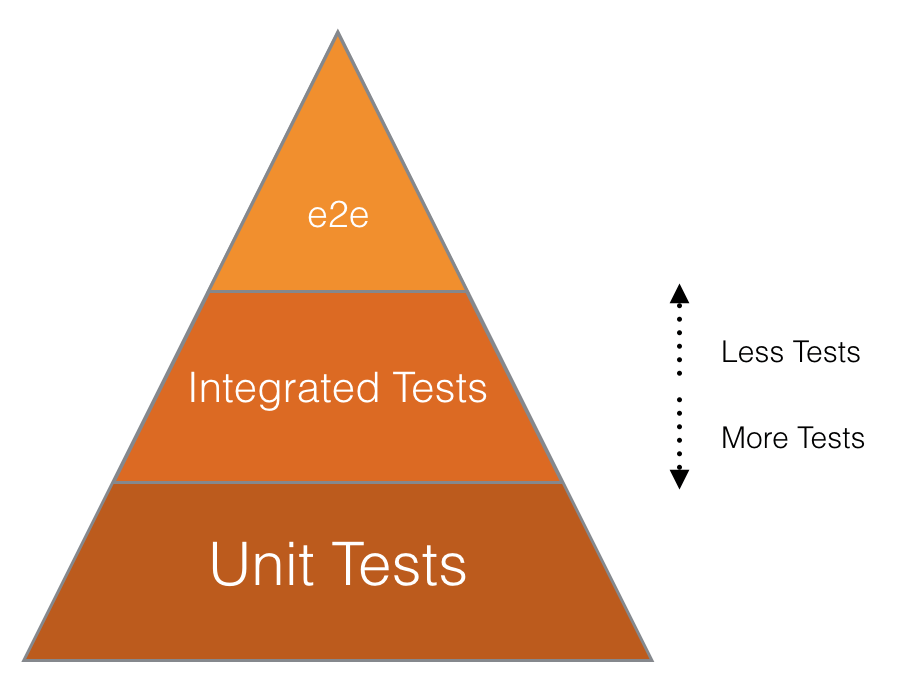
\includegraphics[width=10cm]{images/testing_triangle.png}
    \caption{Piramida testów}
    \label{fig:testing}
\end{figure}

Jak nie trudno było się domyślić znaczną większość testów w kodach programów stanowią testy jednostkowe. Wynika to z dużej popularności metodyki testowania TDD oraz coraz częstszego zauważania przez programistów korzyści wynikających z wykonywania testów. Naturalnym rezultatem chęci zwiększenia procentowego pokrycia kodu testami jest tworzenie większej liczby testów jednostkowych.

Według statystyk opublikowanych przez serwis GitLab\cite{GitLabTesting} testy jednostkowe stanowią na dzień 01.05.2019 71\% wszystkich testów odnalezionych w kodzie. Testy integracyjne oraz White Box pozostają umiarkowanie popularne, natomiast obecność testów Black Box wynosi jedynie 0.17\%.

\begin{center}
\begin{tabular}{ |c|c| } 
 \hline
 Poziom testowania & Ilość testów  \\ 
  \hline
 Testy Black-box (e2e)  & 99 (0.17\%) \\ 
 Testy White-box  & 6440 (10.9\%) \\ 
 Testy integracyjne & 10,577 (17.9\%)  \\ 
 Testy jednostkowe & 41,809 (71\%)  \\ 
 \hline
\end{tabular}
\end{center}

Biorąc pod uwagę, że znaczną większość przeprowadzanych testów stanowią w kodzie testy jednostkowe oraz integracyjne ważne okazują się metody ich automatyzacji. Wykorzystana do tego zostanie praktyka CI - Continuous Integration. 

\subsection{Rola CI w testach}
Zaczynając myślenie o Continuous Integration trzeba najpierw zrozumieć, że nie jest możliwe jednoznaczne zdefiniowanie jak taka ciągła integracja będzie wyglądać w każdym projekcie. Nasze oczekiwania i wymagania od takiej integracji często będą zależne od rodzaju projektu przy którym pracujemy, struktury firmy, wymagań biznesowych od klienta, od faktu czy nasz projekt działa na zasadzie Open Source. Wynika to z faktu, że obecnie ciągła integracja wykorzystywana jest znacznie szerzej niż tylko przeprowadzanie testów w kodzie. 

Ciągła integracja ma pozwolić zespołowi deweloperów na łatwiejsze i bezpieczniejsze tworzenie kodu, podczas którego nie będzie konieczności poświęcania dużej ilości czasu na zarządzanie bazą kodu oraz rozwiązywanie problemów, które wynikają z jednego błędu, a który dotyka dużej części systemu. W praktyce głównym celem do którego dążymy implementując ciągłą integrację jest stworzenie systemu, który po każdym dodaniu kodu do repozytorium będzie uruchamiać wszystkie wyznaczone przez nas testy - zwykle jednostkowe i integracyjne oraz sprawdzi czy dodawany kod spełnia wszystkie narzucone mu wymagania. 

Warto pamiętać, że sam fakt korzystania z systemu zarządzania wersjami, jakim jest git, można potraktować jako ważny element ciągłej integracji. Bez wykorzystania jednego repozytorium kodu dla całego projektu, zarządzanie nim byłoby znacznie bardziej czasochłonne, skomplikowane, a co za tym idzie podatne na powstawanie błędów i różnorakich problemów. Tworzenie projektów przy udziale więcej niż kilku osób mogłoby wymagać więcej czasu na ręczne wysyłanie i łączenie kodu niż samo jego pisanie. 

Jedną z praktyk wykorzystywaną w CI jest częste publikowanie naszych zmian w kodzie do repozytorium. Najczęściej będzie to przynajmniej jeden raz na każdy dzień pracy programisty. Podejście takie sprawia, że łatwiej wykryć jest ewentualne problemy, które mogą pojawić się po naszych zmianach. W przypadku gdy publikowana jest większa ilość kodu, znalezienie przyczyny problemu może byś skomplikowane. Dodatkowo częste publikowanie zmian oznacza, że łatwiej jest połączyć kod pisany w jednym miejscu w pliku przez kilku różnych programistów w procesie "mergowania" zmian. 

Częste publikowanie zmian powoduje też, że kod można łatwiej ze sobą połączyć, w zasadzie jest on zwykle łączony z resztą kodu przez cały swój cykl życia. Aby umożliwić taką sytuację developerzy stają się często pracować tylko na jednej gałęzi deweloperskiej, a gdy nie jest to możliwe wykorzystują gałęzie dedykowane danej funkcjonalności przez jak najkrótszy możliwy czas, aby móc jak najszybciej w jak największym stopniu integrować ich kod z resztą. Dodatkową zaletą szybkiej integracji nowej funkcjonalności jest umożliwienie lepszego i szybszego reagowania na ewentualne zmiany w specyfikacji lub kierunku rozwoju projektu. Stworzona funkcjonalność może być na bieżąco testowana przez osoby odpowiedzialne za tworzenie specyfikacji. W razie zmiany strategii tworzenia projektu będzie można stosunkowo szybko wprowadzić odpowiednie zmiany bez marnowania zbędnie dużej ilości czasu zespołu.

Dużą zaletą wynikającą ze stosowania ciągłej integracji jest znaczne ułatwienie skalowania. Dotyczy to zarówno skalowania projektu jako kod, ale także jako zespół programistyczny. Dobrze przetestowany i przemyślany kod ma szansę być znacznie łatwiej rozbudowywalny od takiego, który nie powstawał w wyniku stosowania dobrych praktyk programistycznych. 

Ułatwienie skalowania zespołu wynika z łatwiejszego wdrażania nowych członków do projektu, dotyczy te szczególnie osób na stanowiskach juniorskich. Kod dodawany przez takie osoby często musiał przechodzić przez recenzję od osoby na stanowisku seniora w celu upewnienia się, że spełnia on oczekiwane standardy. Wykorzystanie Continuous Integration w znacznym stopniu wspomaga taki proces, poprzez wykorzystanie następujących funkcji: 

\begin{itemize}
    \item Automatyczne przeprowadzanie testów 
    
    Jest to podstawowe zadanie praktycznie każdej implementacji Continuous Integration. Zapewnia to możliwość uniknięcia regresji podczas dodawania nowego kodu oraz utrzymywania starego. 
    Platforma na której dokonujemy integracji może zostać skonfigurowana, aby nie pozwolić na dodanie do repozytorium kodu, który nie przejdzie określonych testów. Zwykle będą to wszystkie testy jednostkowe, integracyjne oraz wybrane testy e2e, aktywowane w kodzie przez specjalne flagi, oznaczające elementy projektu, które powinny być poprawnie zaimplementowane,
    \item Sprawdzanie pokrycia kodu testami
    
    Pokrycie testami ( code coverage ) to bardzo ważna statystyka. Wyraża ona w punktach procentowych jak duża część wyrażeń w naszym projekcie jest testowana. Statystykę tę można wykorzystać, w razie gdyby ktoś próbował dodać do repozytorium nieprzetestowany kod. Oczywiście możliwe jest obejście takiego sprawdzenia poprzez napisanie niepoprawnego testu, który nie wnosi żadnej wartości, jednak w dobrych zespołach programistycznych statystyka jest pomocna jeśli chcemy zachować dobrą jakość pisanego kodu. Istnieją opinie, że pokrycie testami powinno wynosić 100\%, jednak zwykle spotykają się one z opinią, że nie przyniesie to wymiernych rezultatów, ponieważ nawet wtedy w programie mogą znaleźć się błędy logiczne, których nie da się wykryć automatycznymi testami. Zwykle przyjmuje się wartości 80\% - 95\% za odpowiednie przy szacowaniu wymaganego pokrycia kodu. Znalezienie odpowiedniej pracy dla naszego projektu wymaga doświadczenia, znajomości zespołu i zrozumienia wymagań jakie stawia przed nami projekt,
    \item Linting kodu
    
    Lintingiem kodu nazywamy wykorzystanie narzędzie do statycznej analizy kodu. Jego zadaniem w przypadku wykorzystania do ciągłej integracji jest sprawdzanie czy kod, który próbujemy dodać odpowiada standardom wykorzystywanym w projekcie. Może to dotyczyć między innymi tego czy nawiasy otwieramy w nowej linii, konwencji tworzenia nazw zmiennych ( wykorzystanie camelCase, PascalCase, podkreślenia ), definiowania argumentów funkcji w wielu liniach. Z pozoru rola lintingu wydaje się mała, a nawet zbędna, jednakże w dużych projektach, przy których pracuje wiele osób o różnych preferencjach ważne jest tworzenie kodu, który jest jednolity stylistycznie, aby był on spójny i łatwy w czytaniu dla osób, które nie mają z nim dużego doświadczenia,
    \item Integracja z kanałem komunikacji
    
    Wykorzystanie Continuous Integration umożliwia synchronizację naszego repozytorium z wykorzystywanym w projekcie kanałem komunikacyjnym. Obecnie najpopularniejszym wykorzystywanym w profesjonalnych projektach jest Slack, a w projektach tworzonych przez społeczność często także Discord. Integracja taka umożliwia nam otrzymywanie na naszym kanale powiadomień dotyczących repozytorium. Możemy skonfigurować je aby otrzymywać je za każdym razem kiedy nie uda się wykonać testu przy próbie dodania kodu. Możliwe będzie wtedy szybsze naprawienie problemu, jeśli powiadomienie otrzymają odpowiednie osoby i będą mogły szybciej zareagować. Powiadomienia możemy wysyłać też przy poprawnym przejściu testów, co może się przydać jeśli wykonujemy skomplikowane testy, których wykonanie zajmuje więcej czasu. 
\end{itemize}

\begin{figure}[htbp]
    \centering
    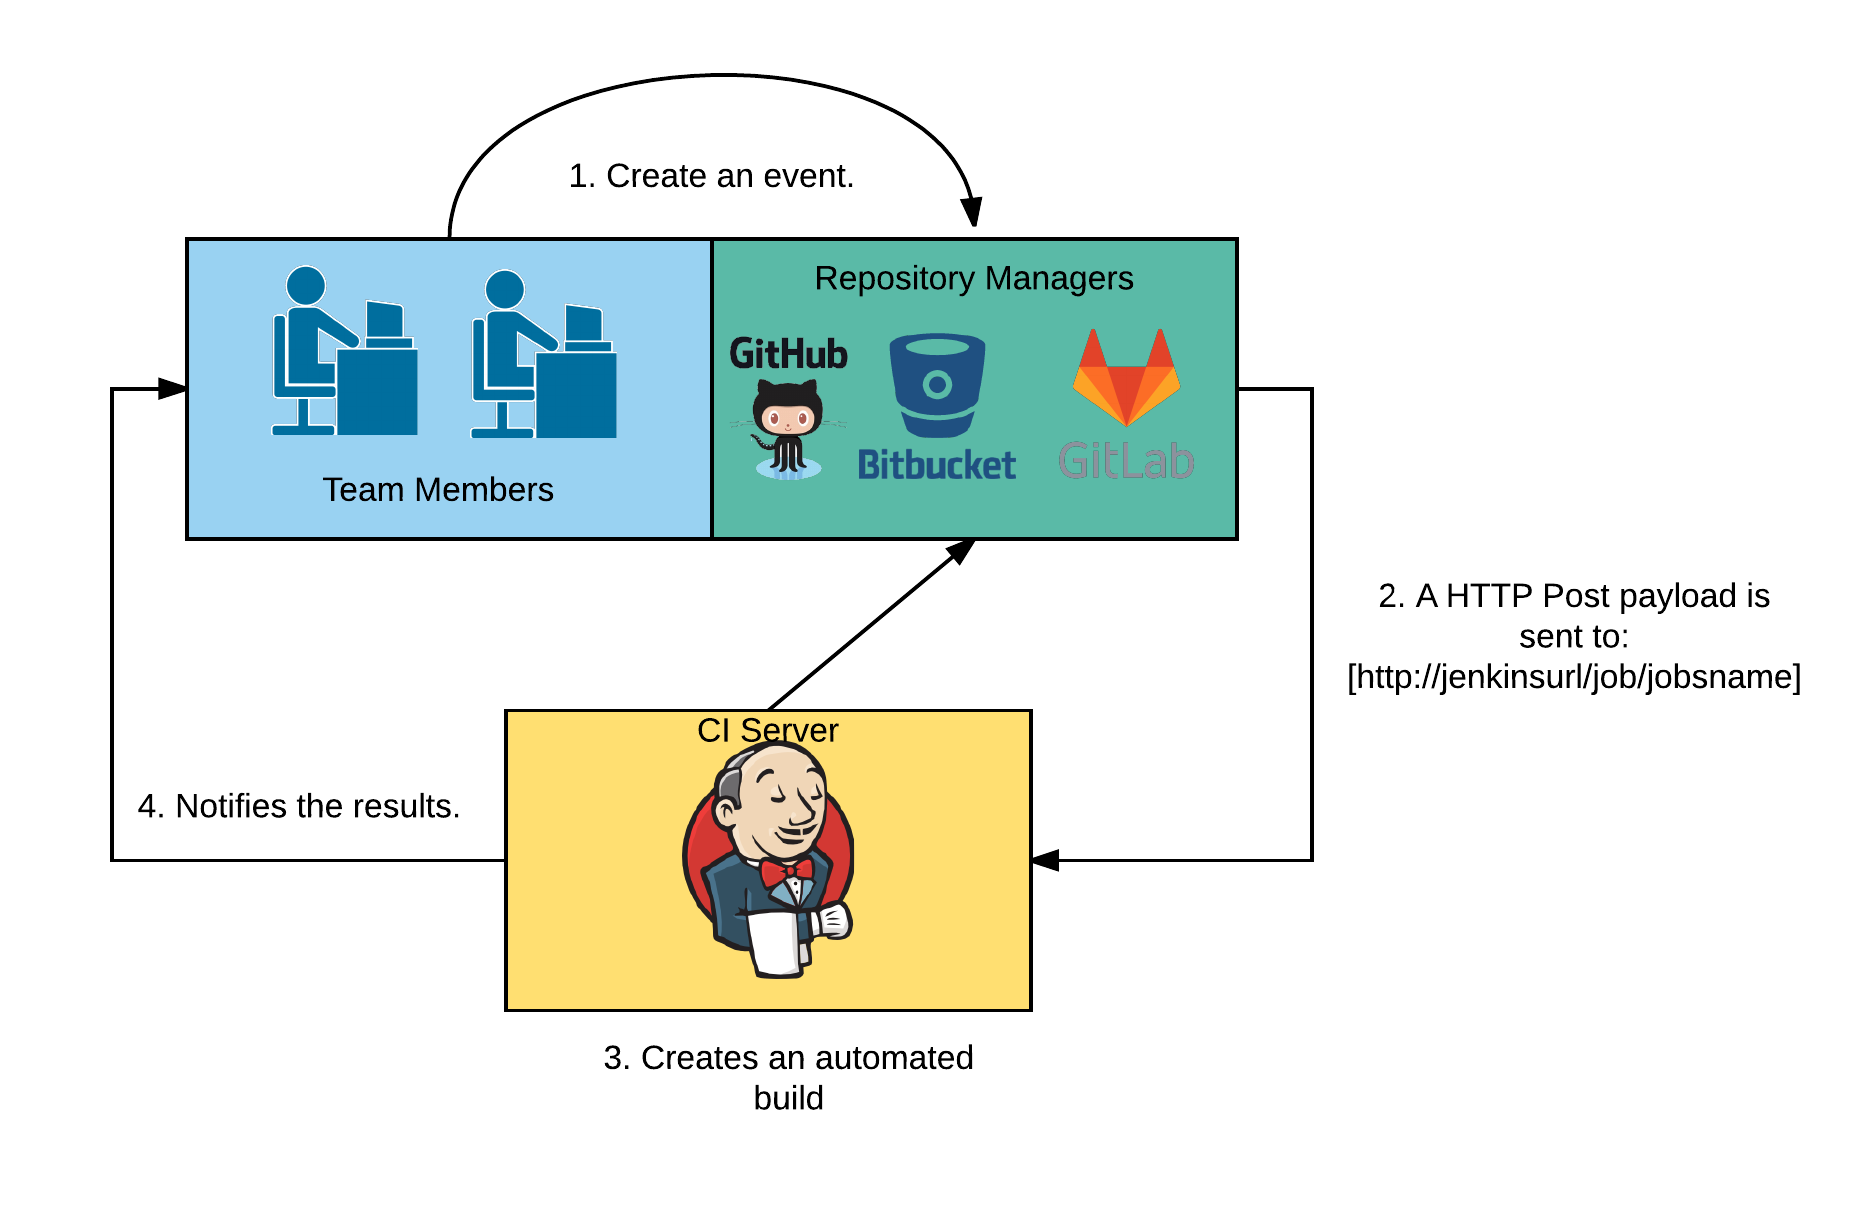
\includegraphics[width=13cm]{images/ci_flow.png}
    \caption{Schemat działania CI, źródło: medium.com/@automationdiscovery}
    \label{fig:ciflow}
\end{figure}

\subsubsection{Wykrywanie błędów bezpieczeństwa}
Dużą korzyścią wynikającą z ciągłej integracji jest możliwość otrzymywania powiadomień dotyczących problemów z bezpieczeństwem w naszym projekcie. Mogą one dotyczyć zarówno błędów wykrytych w wykorzystywanych bibliotekach zewnętrznych jak i przykładowo prywatnych kluczy API, których nie powinniśmy udostępniać publicznie w repozytorium. 

W przypadku wykorzystania platformy GitHub jako repozytorium otrzymujemy alerty o błędach bezpieczeństwa w bibliotekach bez konieczności jakiejkolwiek konfiguracji. 

\begin{figure}[htbp]
    \centering
    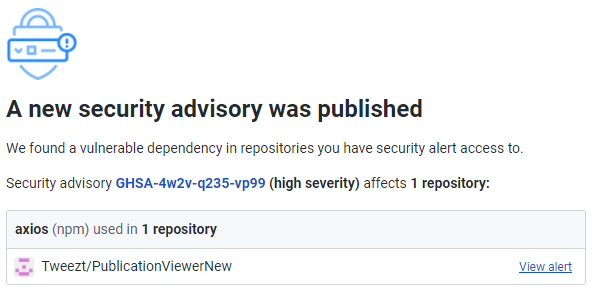
\includegraphics[width=10cm]{images/GitHubAlert.png}
    \caption{Powiadomienie bezpieczeństwa z serwisu GitHub, źródło: własne}
    \label{fig:githubalert}
\end{figure}

Dostępne są także alternatywne serwisy monitorujące repozytoria. Wykorzystanie ich może być konieczne w przypadku projektów komercyjnych, których repozytoria nie są publicznie dostępne. Jednym z popularniejszych jest GitGuardian, który umożliwi nam indywidualne dostosowanie go do potrzeb naszego projektu. 

\begin{figure}[htbp]
    \centering
    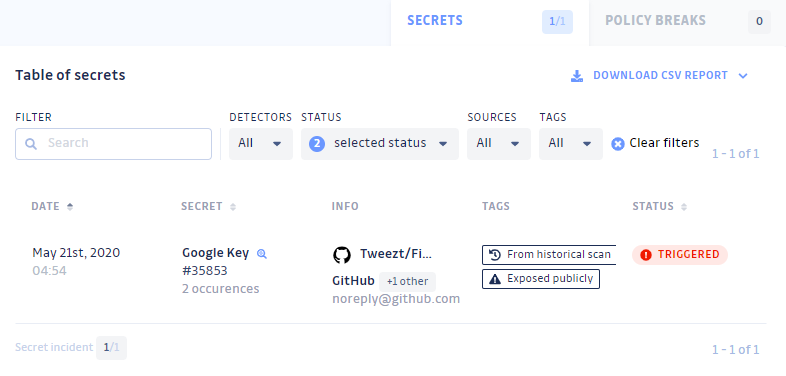
\includegraphics[width=13cm]{images/GitGuardian.png}
    \caption{Powiadomienie bezpieczeństwa z serwisu GitGuardian, źródło: własne}
    \label{fig:gitguardian}
\end{figure}

\subsection{Przykład CI w GitHub Actions}
W celu przetestowania działania różnych funkcjonalności CI do testowania kodu wykorzystamy język python, platformę GitHub oraz oferowaną przez nią usługę GitHub Actions, której działanie zostało już opisane we wcześniejszych częściach pracy.

Nasz projekt spełniać ma następujące założenia: 
\begin{itemize}
    \item Automatycznie wykonywane są wszystkie testy. Do napisania ich wykorzystany zostanie framework pytest. Innym popularnym wyborem dla języka python jest framework unittest. Wybór padł na ten pierwszy ponieważ proste testy można w nim napisać w nieco łatwiejszy sposób, przeszukuje on automatycznie całą bazę kodu w poszukiwaniu testów i umożliwia szybkie uruchomienie ich jedną komendą. Ponadto większość testów pisanych dla unittest zadziała prawidłowo w pytest,
    \item Automatycznie wykonywane jest sprawdzenie pokrycia testami naszego kodu. Wykorzystana zostanie do tego platforma Codecov, która została wybrana z uwagi na łatwą możliwość połączenia z GitHub Actions,
    \item Projekt zintegrowany jest z kanałem Slack, na który wysyłane są powiadomienia o działaniach w repozytorium. Slack został wybrany z uwagi na możliwość łatwej integracji z GitHub Actions oraz swoją popularność przy wykorzystaniu w projektach informatycznych. 
\end{itemize}

Pierwszym krokiem było stworzenie repozytorium z kodem i przygotowanymi dla niego testami. 

\begin{figure}[htbp]
    \centering
    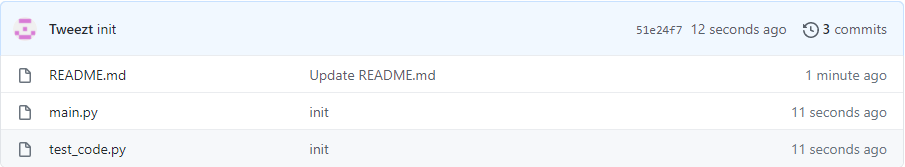
\includegraphics[width=13cm]{images/testingCI1.png}
    \caption{Stworzone repozytorium z przykładowym kodem, źródło: własne}
    \label{fig:ci1}
\end{figure}

\subsubsection{Automatyczne przeprowadzanie testów}
W celu automatycznego wykonywania testów po każdym dodaniu kodu do repozytorium konieczne jest stworzenie tak zwanego workflow. Szczegółowy opis tego zagadnienia został przedstawiony w rozdziale 4.2. 

\begin{lstlisting}[caption={plik main.yaml zawierający workflow automatycznie przeprowadzający testy}]
name: CI
on:
  push:
    branches: [ main ]
  pull_request:
    branches: [ main ]

jobs:
  runtests:
    runs-on: ubuntu-latest

    steps:
      - uses: actions/checkout@v2

      - name: Setup Python
        uses: actions/setup-python@v2.2.1
        with: 
          python-version: 3.8 

      - name: Run tests
        run: |
          pip install pytest
          pytest
\end{lstlisting}

Wykorzystany został w nim system operacyjny Ubuntu w najnowszej wersji oraz język python w wersji 3.8, ponieważ na takiej wersji były przeprowadzane testy lokalne. Samo wykonanie testów odbywa się w dwóch ostatnich liniach. Najpierw instalowana jest biblioteka pytest, a następnie jednym poleceniem uruchamiane są wszystkie zaimplementowane w kodzie testy. 

\begin{figure}[htbp]
    \centering
    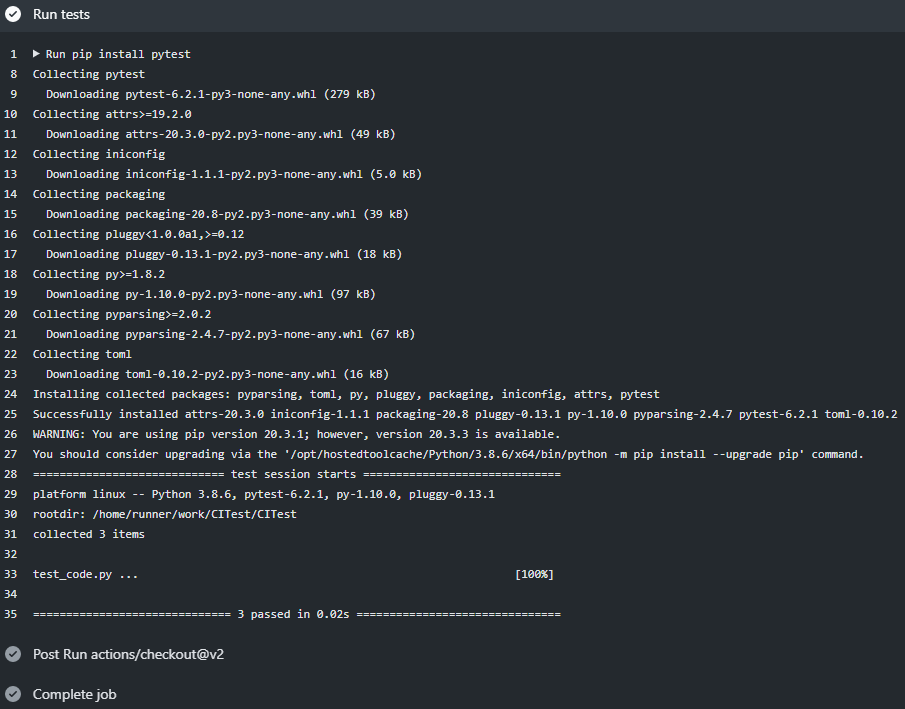
\includegraphics[width=11cm]{images/testingCI3.png}
    \caption{Wynik uruchomionej akcji z testami, źródło: własne}
    \label{fig:ci3}
\end{figure}

Po przejściu do zakładki Actions, można zobaczyć, że testy wykonane zostały poprawnie. 
Po celowym sprawieniu, że test jednostkowy nie powodzi się i opublikowaniu zmian w repozytorium można zobaczyć że jesteśmy o tym informowani w zakładce Actions oraz nad listą plików w repozytorium. 

\begin{figure}[htbp]
    \centering
    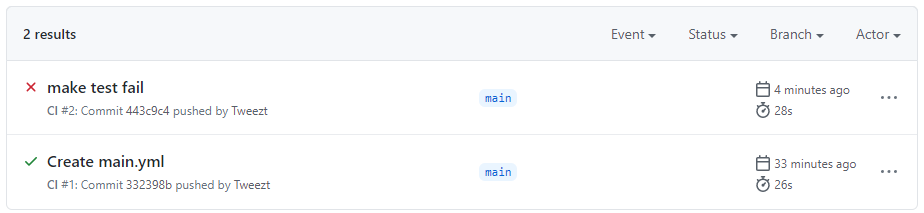
\includegraphics[width=11cm]{images/testingCI4.png}
    \caption{Negatywny wynik testu w zakładce Actions, źródło: własne}
    \label{fig:ci4}
\end{figure}

\begin{figure}[htbp]
    \centering
    
\includegraphics[width=7cm]{images/testingCI5.png}
    \caption{Negatywny wynik testu nad listą plików, źródło: własne}
    \label{fig:ci5}
\end{figure}

\subsubsection{Integracja z serwisem Codecov}
Pierwszym krokiem do przeprowadzenia integracji z serwisem Codecov było zalogowanie się tam przy pomocy konta GitHub, na którym znajduje się repozytorium z projektem. Po udanym zalogowaniu konieczne było pobranie klucza CODECOV\_TOKEN, który należy umieścić w odpowiednim miejscu w ustawieniach repozytorium. Kolejnym krokiem było utworzenie kolejnego pliku .yaml odpowiedzialnego za uruchamianie nowego workflow. 

\begin{lstlisting}[caption={plik coverage.yaml zawierający workflow automatycznie sprawdzający pokrycie testami}]
name: coverage testing
on:
  push:
    branches: [ main ]
    
jobs:
  runtests:
    runs-on: ubuntu-latest
    steps:
      - uses: actions/checkout@v2

      - name: Setup Python
        uses: actions/setup-python@v2.2.1
        with: 
          python-version: 3.8 
      - name: Generate coverage report
        run: |
          pip install pytest
          pip install pytest-cov
          coverage run test_code.py
          coverage report
          coverage xml
      - name: Upload  to Codecov
        uses: codecov/codecov-action@v1
        with:
          token: ${{ secrets.CODECOV_TOKEN }}
          file: ./coverage.xml
          flags: unittests
\end{lstlisting}

Wykorzystywana jest tutaj akcja codecov-action, która pozwala nam w łatwy sposób automatycznie wysłać nasz raport do serwisu. Po prawidłowym wykonaniu wszystkich operacji możemy zobaczyć nasze pokrycie testami w serwisie Codecov.io. 

\begin{figure}[htbp]
    \centering
    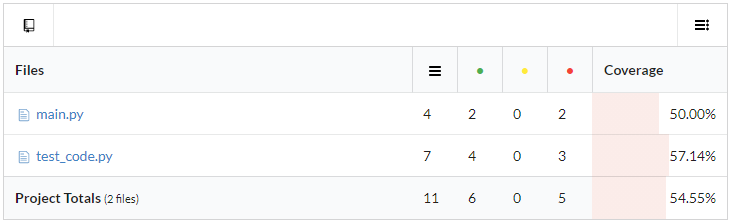
\includegraphics[width=12cm]{images/testingCI6.png}
    \caption{Raport pokrycia kodu testami, źródło: własne}
    \label{fig:ci6}
\end{figure}

\subsubsection{Integracja z kanałem Slack}
Integrację z kanałem Slack można przeprowadzić w sposób analogiczny do integracji z serwisem Codecov, pomocne są tutaj Akcje dostarczone przez te serwisy, które powodują, że konieczna konfiguracja sprowadza się do podania odpowiednich kluczy dostępu. Z tego powodu wykorzystamy odmienne podejście, aby sprawdzić jak można dokonać takiej integracji od strony Slacka. 

Pierwszym krokiem było dodanie aplikacji GitHub do naszego kanału Slack. Można ją znaleźć w galerii aplikacji, dostępnej pod adresem \url{citestingworkspace.slack.com/apps}. Po poprawnym uwierzytelnieniu konta należy wybrać, do których kanałów chcemy dać aplikacji dostęp. 

\begin{figure}[htbp]
    \centering
    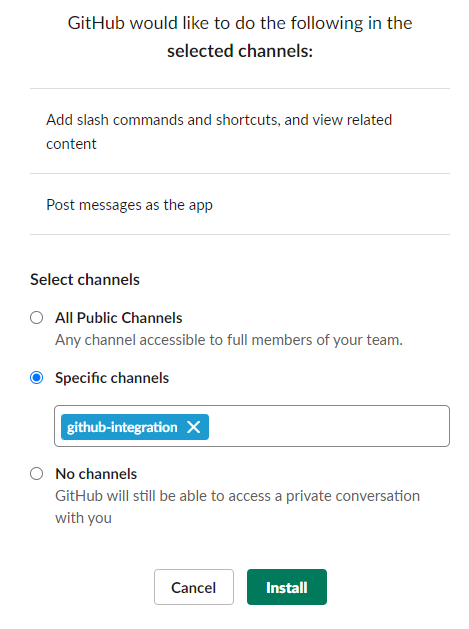
\includegraphics[width=5cm]{images/testingCI7.png}
    \caption{Nadanie aplikacji GitHub uprawnień do korzystania z kanałów, źródło: własne}
    \label{fig:ci7}
\end{figure}
Ostatnim krokiem jak wskazanie aplikacji, z którym repozytorium w serwisie GitHub chcemy ją zintegrować. Odbywa się to poprzez polecenie 
\begin{lstlisting}[caption={Polecenie pozwalające połączyć aplikację GitHub z repozytorium}]
/github subscribe owner/repository
\end{lstlisting}

gdzie owner to nazwa konta, a repository to nazwa naszego repozytorium. 

Po wykonaniu wszystkich kroków i udostępnieniu nowej zmiany w repozytorium możemy zobaczyć powiadomienie wysłane nam przez nowo zainstalowaną aplikację. 

\begin{figure}[htbp]
    \centering
    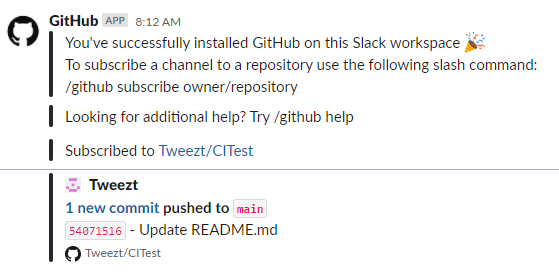
\includegraphics[width=12cm]{images/testingCI9.png}
    \caption{Powiadomienie o nowych zmianach w kodzie w repozytorium, źródło: własne}
    \label{fig:ci9}
\end{figure}

Po wykonaniu wszystkich tych czynności udało nam się stworzyć repozytorium, które dzięki wykorzystaniu ciągłej integracji pozwala na sprawne przeprowadzanie testów, analizę pokrycia nimi kodu oraz umożliwia automatyczne informowanie członków zespołu o zmianach w kodzie. 


\section{Podsumowanie i wnioski}
Pisząc naszą pracę chcieliśmy zgromadzić jak największą ilość wiedzy oraz dobrych praktyk, dotyczących nowoczesnych metod tworzenia oprogramowania. Z tego też powodu pracę otworzyliśmy rozdziałem wprowadzającym, w którym przybliżyliśmy jak istotną rolę w dzisiejszym przemyśle informatycznym odgrywa automatyzacja procesów. Dużą część naszej pracy stanowi teoria, ponieważ uważamy, że zrozumienie idei jest pierwszym i być może najistotniejszym krokiem, dzięki któremu nasza praca przy automatyzacji będzie skuteczna.

Automatyzacja jest stosowana powszechnie w praktycznie każdym zespole programistycznym. Z powodu jej powszechności i dostępności materiałów do nauki coraz częściej implementowana jest też przez programistów w prywatnych projektach, ponieważ widzą oni wartość dodaną, która ona wnosi. 

My również zauważyliśmy takie korzyści, dlatego podczas pisania pracy zdecydowaliśmy się na implementację zasady CI/CD, dzięki której nasz plik \LaTeX{} po opublikowaniu zmian w repozytorium automatycznie budował się i publikował w formacie .pdf na stronie internetowej w formie łatwej do czytania. 

\begin{figure}[htbp]
    \centering
    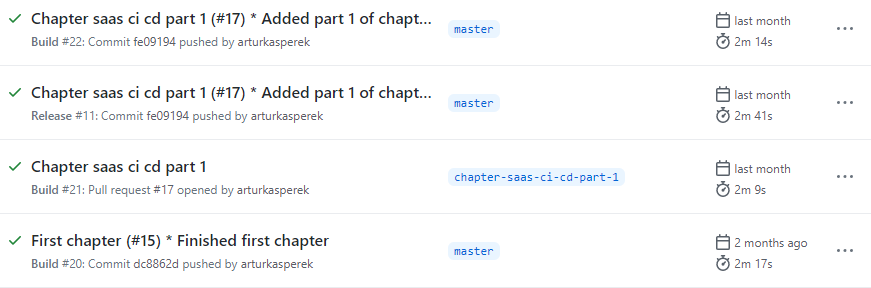
\includegraphics[width=12cm]{images/podsumowanie.png}
    \caption{Budowanie nowych wersji naszej pracy, źródło: własne}
    \label{fig:podsumowanie}
\end{figure}

W pracy przedstawiliśmy jak rozwijała się automatyzacja procesów w przeszłości oraz jakie praktyki możliwe są do zastosowania współcześnie. Przedstawiliśmy narzędzia, które ułatwiają takie procesy 

Podejście CI/CD pozwala programistom na efektywne wykonywanie swoich obowiązków. Eliminowane są zbędne przestoje w pracy, problemy wynikające z regresji w kodzie, a same nowe funkcjonalności publikowane są szybciej. Ciągłe testowanie wzmacnia pewność siebie programisty, nie musi się on martwić, że jego zmiany spowodują problemy dla reszty członków zespołu, w najgorszym wypadku jego zmiany nie zostaną zaakceptowane. 

Uważamy, że temat naszej pracy można jeszcze zdecydowanie pogłębić, ponieważ jest to dziedzina dynamicznie rozwijająca się, a zapotrzebowanie na taką automatyzację powinno tylko rosnąć w przyszłości. Możliwa byłaby przykładowo analiza innych platform programistycznych, szczególnie nowo powstających oraz odmiennych metod tworzenia oprogramowania. Uważamy, że warto interesować się zagadnieniami automatyzacji w programowaniu, ponieważ wykorzystanie jej staje się standardem w praktycznie każdej firmie w branży IT.

\begin{thebibliography}{12}

\bibitem{AgileManifesto} Kent Beck; James Grenning; Robert C. Martin; Mike Beedle; Jim Highsmith; Steve Mellor; Arie van Bennekum; Andrew Hunt; Ken Schwaber; Alistair Cockburn; Ron Jeffries; Jeff Sutherland; Ward Cunningham; Jon Kern; Dave Thomas; Martin Fowler; Brian Marick (2001). "Principles behind the Agile Manifesto"
\bibitem{DevOpsBook} Bass, Len; Weber, Ingo; Zhu, Liming (2015). DevOps: A Software Architect's Perspective

\end{thebibliography}
\end{document}
